% Options for packages loaded elsewhere
% Options for packages loaded elsewhere
\PassOptionsToPackage{unicode}{hyperref}
\PassOptionsToPackage{hyphens}{url}
\PassOptionsToPackage{dvipsnames,svgnames,x11names}{xcolor}
%
\documentclass[
  letterpaper,
  DIV=11,
  numbers=noendperiod]{scrartcl}
\usepackage{xcolor}
\usepackage{amsmath,amssymb}
\setcounter{secnumdepth}{-\maxdimen} % remove section numbering
\usepackage{iftex}
\ifPDFTeX
  \usepackage[T1]{fontenc}
  \usepackage[utf8]{inputenc}
  \usepackage{textcomp} % provide euro and other symbols
\else % if luatex or xetex
  \usepackage{unicode-math} % this also loads fontspec
  \defaultfontfeatures{Scale=MatchLowercase}
  \defaultfontfeatures[\rmfamily]{Ligatures=TeX,Scale=1}
\fi
\usepackage{lmodern}
\ifPDFTeX\else
  % xetex/luatex font selection
\fi
% Use upquote if available, for straight quotes in verbatim environments
\IfFileExists{upquote.sty}{\usepackage{upquote}}{}
\IfFileExists{microtype.sty}{% use microtype if available
  \usepackage[]{microtype}
  \UseMicrotypeSet[protrusion]{basicmath} % disable protrusion for tt fonts
}{}
\makeatletter
\@ifundefined{KOMAClassName}{% if non-KOMA class
  \IfFileExists{parskip.sty}{%
    \usepackage{parskip}
  }{% else
    \setlength{\parindent}{0pt}
    \setlength{\parskip}{6pt plus 2pt minus 1pt}}
}{% if KOMA class
  \KOMAoptions{parskip=half}}
\makeatother
% Make \paragraph and \subparagraph free-standing
\makeatletter
\ifx\paragraph\undefined\else
  \let\oldparagraph\paragraph
  \renewcommand{\paragraph}{
    \@ifstar
      \xxxParagraphStar
      \xxxParagraphNoStar
  }
  \newcommand{\xxxParagraphStar}[1]{\oldparagraph*{#1}\mbox{}}
  \newcommand{\xxxParagraphNoStar}[1]{\oldparagraph{#1}\mbox{}}
\fi
\ifx\subparagraph\undefined\else
  \let\oldsubparagraph\subparagraph
  \renewcommand{\subparagraph}{
    \@ifstar
      \xxxSubParagraphStar
      \xxxSubParagraphNoStar
  }
  \newcommand{\xxxSubParagraphStar}[1]{\oldsubparagraph*{#1}\mbox{}}
  \newcommand{\xxxSubParagraphNoStar}[1]{\oldsubparagraph{#1}\mbox{}}
\fi
\makeatother


\usepackage{longtable,booktabs,array}
\usepackage{calc} % for calculating minipage widths
% Correct order of tables after \paragraph or \subparagraph
\usepackage{etoolbox}
\makeatletter
\patchcmd\longtable{\par}{\if@noskipsec\mbox{}\fi\par}{}{}
\makeatother
% Allow footnotes in longtable head/foot
\IfFileExists{footnotehyper.sty}{\usepackage{footnotehyper}}{\usepackage{footnote}}
\makesavenoteenv{longtable}
\usepackage{graphicx}
\makeatletter
\newsavebox\pandoc@box
\newcommand*\pandocbounded[1]{% scales image to fit in text height/width
  \sbox\pandoc@box{#1}%
  \Gscale@div\@tempa{\textheight}{\dimexpr\ht\pandoc@box+\dp\pandoc@box\relax}%
  \Gscale@div\@tempb{\linewidth}{\wd\pandoc@box}%
  \ifdim\@tempb\p@<\@tempa\p@\let\@tempa\@tempb\fi% select the smaller of both
  \ifdim\@tempa\p@<\p@\scalebox{\@tempa}{\usebox\pandoc@box}%
  \else\usebox{\pandoc@box}%
  \fi%
}
% Set default figure placement to htbp
\def\fps@figure{htbp}
\makeatother


% definitions for citeproc citations
\NewDocumentCommand\citeproctext{}{}
\NewDocumentCommand\citeproc{mm}{%
  \begingroup\def\citeproctext{#2}\cite{#1}\endgroup}
\makeatletter
 % allow citations to break across lines
 \let\@cite@ofmt\@firstofone
 % avoid brackets around text for \cite:
 \def\@biblabel#1{}
 \def\@cite#1#2{{#1\if@tempswa , #2\fi}}
\makeatother
\newlength{\cslhangindent}
\setlength{\cslhangindent}{1.5em}
\newlength{\csllabelwidth}
\setlength{\csllabelwidth}{3em}
\newenvironment{CSLReferences}[2] % #1 hanging-indent, #2 entry-spacing
 {\begin{list}{}{%
  \setlength{\itemindent}{0pt}
  \setlength{\leftmargin}{0pt}
  \setlength{\parsep}{0pt}
  % turn on hanging indent if param 1 is 1
  \ifodd #1
   \setlength{\leftmargin}{\cslhangindent}
   \setlength{\itemindent}{-1\cslhangindent}
  \fi
  % set entry spacing
  \setlength{\itemsep}{#2\baselineskip}}}
 {\end{list}}
\usepackage{calc}
\newcommand{\CSLBlock}[1]{\hfill\break\parbox[t]{\linewidth}{\strut\ignorespaces#1\strut}}
\newcommand{\CSLLeftMargin}[1]{\parbox[t]{\csllabelwidth}{\strut#1\strut}}
\newcommand{\CSLRightInline}[1]{\parbox[t]{\linewidth - \csllabelwidth}{\strut#1\strut}}
\newcommand{\CSLIndent}[1]{\hspace{\cslhangindent}#1}



\setlength{\emergencystretch}{3em} % prevent overfull lines

\providecommand{\tightlist}{%
  \setlength{\itemsep}{0pt}\setlength{\parskip}{0pt}}



 


\usepackage{booktabs}
\usepackage{longtable}
\usepackage{array}
\usepackage{multirow}
\usepackage{wrapfig}
\usepackage{float}
\usepackage{colortbl}
\usepackage{pdflscape}
\usepackage{tabu}
\usepackage{threeparttable}
\usepackage{threeparttablex}
\usepackage[normalem]{ulem}
\usepackage{makecell}
\usepackage{xcolor}
\KOMAoption{captions}{tableheading}
\makeatletter
\@ifpackageloaded{caption}{}{\usepackage{caption}}
\AtBeginDocument{%
\ifdefined\contentsname
  \renewcommand*\contentsname{Table of contents}
\else
  \newcommand\contentsname{Table of contents}
\fi
\ifdefined\listfigurename
  \renewcommand*\listfigurename{List of Figures}
\else
  \newcommand\listfigurename{List of Figures}
\fi
\ifdefined\listtablename
  \renewcommand*\listtablename{List of Tables}
\else
  \newcommand\listtablename{List of Tables}
\fi
\ifdefined\figurename
  \renewcommand*\figurename{Figure}
\else
  \newcommand\figurename{Figure}
\fi
\ifdefined\tablename
  \renewcommand*\tablename{Table}
\else
  \newcommand\tablename{Table}
\fi
}
\@ifpackageloaded{float}{}{\usepackage{float}}
\floatstyle{ruled}
\@ifundefined{c@chapter}{\newfloat{codelisting}{h}{lop}}{\newfloat{codelisting}{h}{lop}[chapter]}
\floatname{codelisting}{Listing}
\newcommand*\listoflistings{\listof{codelisting}{List of Listings}}
\makeatother
\makeatletter
\makeatother
\makeatletter
\@ifpackageloaded{caption}{}{\usepackage{caption}}
\@ifpackageloaded{subcaption}{}{\usepackage{subcaption}}
\makeatother
\usepackage{bookmark}
\IfFileExists{xurl.sty}{\usepackage{xurl}}{} % add URL line breaks if available
\urlstyle{same}
\hypersetup{
  pdftitle={Analysis of iPSC Gene Expression (will be changed)},
  pdfauthor={Trinity Minard},
  colorlinks=true,
  linkcolor={blue},
  filecolor={Maroon},
  citecolor={Blue},
  urlcolor={Blue},
  pdfcreator={LaTeX via pandoc}}


\title{Analysis of iPSC Gene Expression (will be changed)}
\usepackage{etoolbox}
\makeatletter
\providecommand{\subtitle}[1]{% add subtitle to \maketitle
  \apptocmd{\@title}{\par {\large #1 \par}}{}{}
}
\makeatother
\subtitle{Final Project}
\author{Trinity Minard}
\date{2025-12-03}
\begin{document}
\maketitle


\section{Abstract}\label{abstract}

\section{Introduction}\label{introduction}

The discovery of human induced pluripotent stem cells (iPSCs) by
Takahashi and Yamanaka in 2007 (Takahashi et al., 2007) has
revolutionized the regenerative medicine field. iPSCs are created by
reprogramming somatic cells into an embryonic like state using the
Yamanaka transciption factors: SOX2, OCT4, KLF4, and c-Myc). These cells
have vast capabilities due to their ability to model human development
and diseases \emph{in vitro}, and their potential for patient specific
(autologous) and ``off the shelf'' (allogeneic) cell therapies
(Cerneckis et al., 2024).

With that being said, the characterization of iPSC lines is essential in
any experimental or manufacturing process to ensure consistency in
culturing. This includes analyzing the expression of pluripotency (stem
cell) markers, differentiation markers, and potential chromosomal
abnormalies, to access the population of the culture. This is commonly
done using techniques such as reverse transcriptase or real time
quantitative PCR (RT-qPCR) to analyze mRNA expression (Artyukhov et al.,
2017), or using an antibody based experiment to analyze protein
expression levels, such as Flow Cytometry or immunocytochemistry. When
conducting these experiments, specifically RT-qPCR, reference genes,
also known as housekeeping genes, are used to normalize the expression
of other genes in a sample (Artyukhov et al., 2017). This allows the
expression of genes to be compared across different samples, since it is
presumed that the expression of the housekeeping gene is consistent
across all of the samples. In stem cell samples, however, it has been
found that the commonly used housekeeping genes, such as GAPDH, appear
to fluctuate in iPSC samples (Panina et al., 2020), making it difficult
to achieve accurate normalization data.

RNA Seq is a technique that sequences the entirety of RNA molecules in a
given sample, rather than using gene specific primers or probes as in
RT-qPCR and other techniques. This allows the entire transciptome to be
analyzed, providing a complete picture of the expression of genes in a
sample (Wang et al., 2009). Additionally, gene expression is calculated
by dividing the raw counts of a gene by the total counts in a sample,
eliminating the need for a housekeeping gene. This allows for an
unbiased and quantitiative analysis of millions of genes in sample (Wang
et al., 2009). Despite these advantages, RNA-Seq is far more time
consuming and expensive than RT-qPCR and other experiments, making it
non practical in a manufacturing setting. Therefore, utilizing RNA-Seq
to analyze iPSC samples could provide insight into housekeeping gene
expression, allowing researchers to select ideal reference genes for
their analysis.

A similar study, conducted by Carcamo-Orive \emph{et al.,} investigated
the variability of gene expression across 317 iPSC lines generated from
101 individuals (Carcamo-Orive et al., 2017) and created a publically
avaible data set of their raw RNA Seq data. They found that genetic
variability in the iPSC lines was influenced by a donor specific gene
expression pattern, specifically influenced by donor age, sex, ancestry,
and reprogramming variabilies. iPSCs can also be reprogrammed from a
variety of somatic cells, such as blood, skin fibroblasts, hair
keratinocytes, urine cells, mesencymal stem cells, and bone marrow
(Poetsch et al., 2022). While some somatic cells are easier to obtain
than others, such as blood cells and fibroblasts, iPSCs from these lines
are associated with higher genomic mutations due to the somatic cells'
high turnover rate. Additionally, iPSCs appear to have an epigenetic
memory of their tissue of origin, which has been found to influence
their differentiation (Poetsch et al., 2022). All of these factors, and
many others, could be contributing to the variations in gene expression
in iPSC samples.

This publicly available dataset from Carcamo-Orive \emph{et al.} was
used to analyze the expression of RNA across iPSC samples, with a focus
on the expression of pluripotency markers, differentiation markers, and
housekeeping genes.

\section{Methods}\label{methods}

\subsubsection{Data Cleaning}\label{data-cleaning}

RNA-Seq counts per million data (named: cpm\_data), and sample metadata
(named: raw\_counts) were acquired from Stemformatics using the
Carcamo-Orive (2017) dataset (Carcamo-Orive et al., 2017). Genes in this
study were referred to by their Ensembl ID, so gene information, such as
name and RNA type, was integrated from the Ensembl database. Using R (R
Core Team, 2025), the raw count per million data was converted to a log
base 2 scale with a 0.5 offset to prevent samples with a count of 0 from
becoming skewed. Values for age, from the metadata file, were grouped by
decade, and an additional column was added for an age + sex category
(i.e., 40s female). Information from the sample description was then
extracted to create columns for race and insulin resistance. The
metadata and log₂ counts per million files were then merged into one
data frame for further analysis.

\subsubsection{Category Tables}\label{category-tables}

The number of samples for each group within the age-sex and race
categories were summarized and displayed as two tables using the knitr
(Xie, 2025) and kableExtra (Zhu, 2024) packages.

\subsubsection{Pie Charts by RNA
Category}\label{pie-charts-by-rna-category}

Genes detected in the RNA Seq counts per million data were grouped into
the following categories: Protein coding, long non-coding RNA (lncRNA),
Small RNAs, Pseudogenes, and Other. A count of the number of genes in
each category was then performed by using the dplyr package (Wickham et
al., 2023) from tidyverse (Wickham, 2023). The total expression of each
category was also calculated using the raw count per million data. The
scales (Wickham, Pedersen, et al., 2025) package from ggplot2 (Wickham,
Chang, et al., 2025) was used to create two pie charts, one of the gene
counts and one of the gene expression by RNA category, plotted together
using the patchwork package (Pedersen, 2025).

\subsubsection{Principal Component Analysis (PCA)
Plots}\label{principal-component-analysis-pca-plots}

Log₂ expression values were first cleaned by removing entries without
gene information and duplicate gene names. Gene variances were
calculated across the samples, and genes with no variance were removed.
To visualize the major sources of variation in the expression data, a
principal component analysis (PCA) was performed using the FactoMineR
package (Husson et al., 2025), which identifies the major axes of
variation in the dataset. To assess if sample characteristics (sex, age
decade, combined age sex groups, and race) influenced the PCA's
structure, a Welch's one-way ANOVA, which does not assume equal
variance, was performed separately for PCA1 and PCA2. Significant
differences were found for the age sex groups and race categories, so
two PCA biplots were generated, each overlaying confidence ellipses
corresponding to either age sex groups or race. On both of the biplots,
the top twenty genes with the highest variance across all samples were
labeled and displayed as vectors.

\subsubsection{Pluripotency, Differentiation, and Housekeeping Gene
Expression}\label{pluripotency-differentiation-and-housekeeping-gene-expression}

The log₂ expression of genes, categorized as pluripotency markers,
differentiation markers, and housekeeping genes, was compared across
sample groups (age-sex and race) using heatmaps, linear mixed-effects
models, and Welch's ANOVA with post hoc Games-Howell tests. Heatmaps of
log₂ gene expression were generated using the pheatmap package (Kolde,
2025) to visualize overall expression patterns within each gene
category. Linear mixed-effect models were then fit using lme4 (Bates et
al., 2025) and lmerTest (Kuznetsova et al., 2020) to evaluate
differences in gene expression across age-sex and race groups, while
accounting for gene-specific baseline expression levels by using random
intercepts for genes. Percent differences in overall gene expression
were calculated by exponentiating the estimated log₂ scale coefficient
back to fold change, subtracting one, and multiplying by 100. QQ plots
and histograms were generated, but not shown here, for each model to
view residuals and assess model assumptions. To identify which genes
displayed statistically significant differences in expression between
sample categories, Welch's one-way ANOVA, assuming unequal variance, was
performed for each gene. P values were adjusted using the
Benjamini-Hochberg method due to the high number of tests that were
performed. For genes with significant ANOVA results, Games-Howell post
hoc tests, using rstatix (\textbf{R-statix?}), were performed and
p-values were Benjamini-Hochberg corrected. Significant Games Howell
comparisons (adjusted p \textless{} 0.05) were annotated on bar plots
displaying log₂ expression for each gene across sample groups.

\section{Results}\label{results}

\begin{table}[!h]
\centering
\caption{\label{tab:unnamed-chunk-12}Sample counts by Age-Sex}
\centering
\begin{tabular}[t]{lr}
\toprule
Age-Sex Group & Sample Count\\
\midrule
\cellcolor{gray!10}{40s female} & \cellcolor{gray!10}{34}\\
40s male & 8\\
\cellcolor{gray!10}{50s female} & \cellcolor{gray!10}{63}\\
50s male & 41\\
\cellcolor{gray!10}{60s female} & \cellcolor{gray!10}{77}\\
\addlinespace
60s male & 57\\
\cellcolor{gray!10}{70s female} & \cellcolor{gray!10}{17}\\
70s male & 11\\
\bottomrule
\end{tabular}
\end{table}

\begin{table}[!h]
\centering
\caption{\label{tab:unnamed-chunk-12}Sample counts by Race}
\centering
\begin{tabular}[t]{lr}
\toprule
Race & Sample Count\\
\midrule
\cellcolor{gray!10}{African American} & \cellcolor{gray!10}{20}\\
Asian & 33\\
\cellcolor{gray!10}{Caucasian} & \cellcolor{gray!10}{212}\\
Hispanic & 14\\
\cellcolor{gray!10}{South Asian} & \cellcolor{gray!10}{13}\\
\addlinespace
NA & 16\\
\bottomrule
\end{tabular}
\end{table}

\begin{figure}

\centering{

\pandocbounded{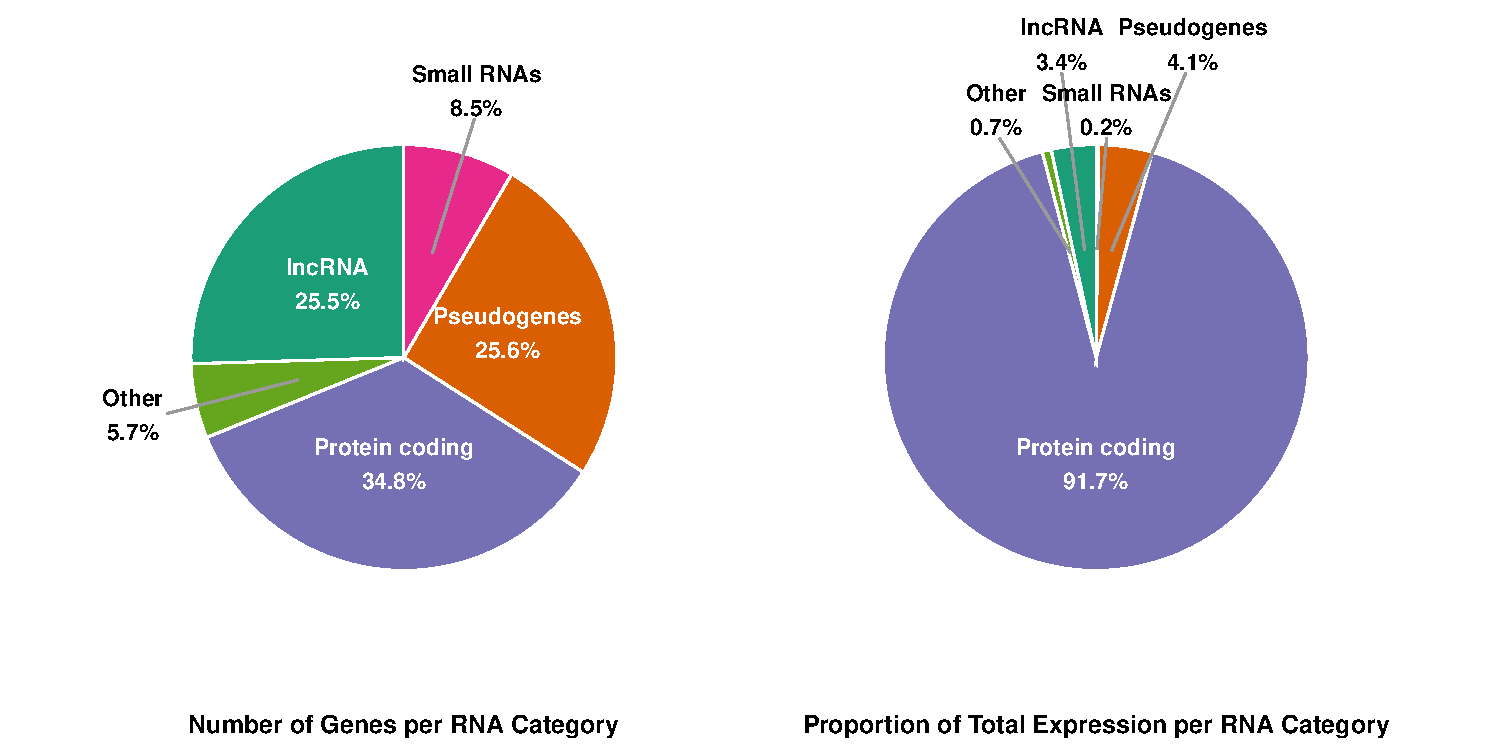
\includegraphics[keepaspectratio]{Final-Project-BIOL806-V4_files/figure-pdf/fig-rna-pie-chart-1.pdf}}

}

\caption{\label{fig-rna-pie-chart}Detected RNA Types in iPSC Samples
Analzyed using RNA Seq. The number of genes detected in each RNA
category from RNA-seq data were counted and plotted as a pie chart
(left). Small categories (\textless{} 2 \%), such as rRNA, tRNA, and
immunoglobulin genes, were combined into an `Other' category. The
expression of genes, using raw count per million data, was averaged by
type of RNA and plotted as a pie chart (right).}

\end{figure}%

\begin{figure}

\centering{

\pandocbounded{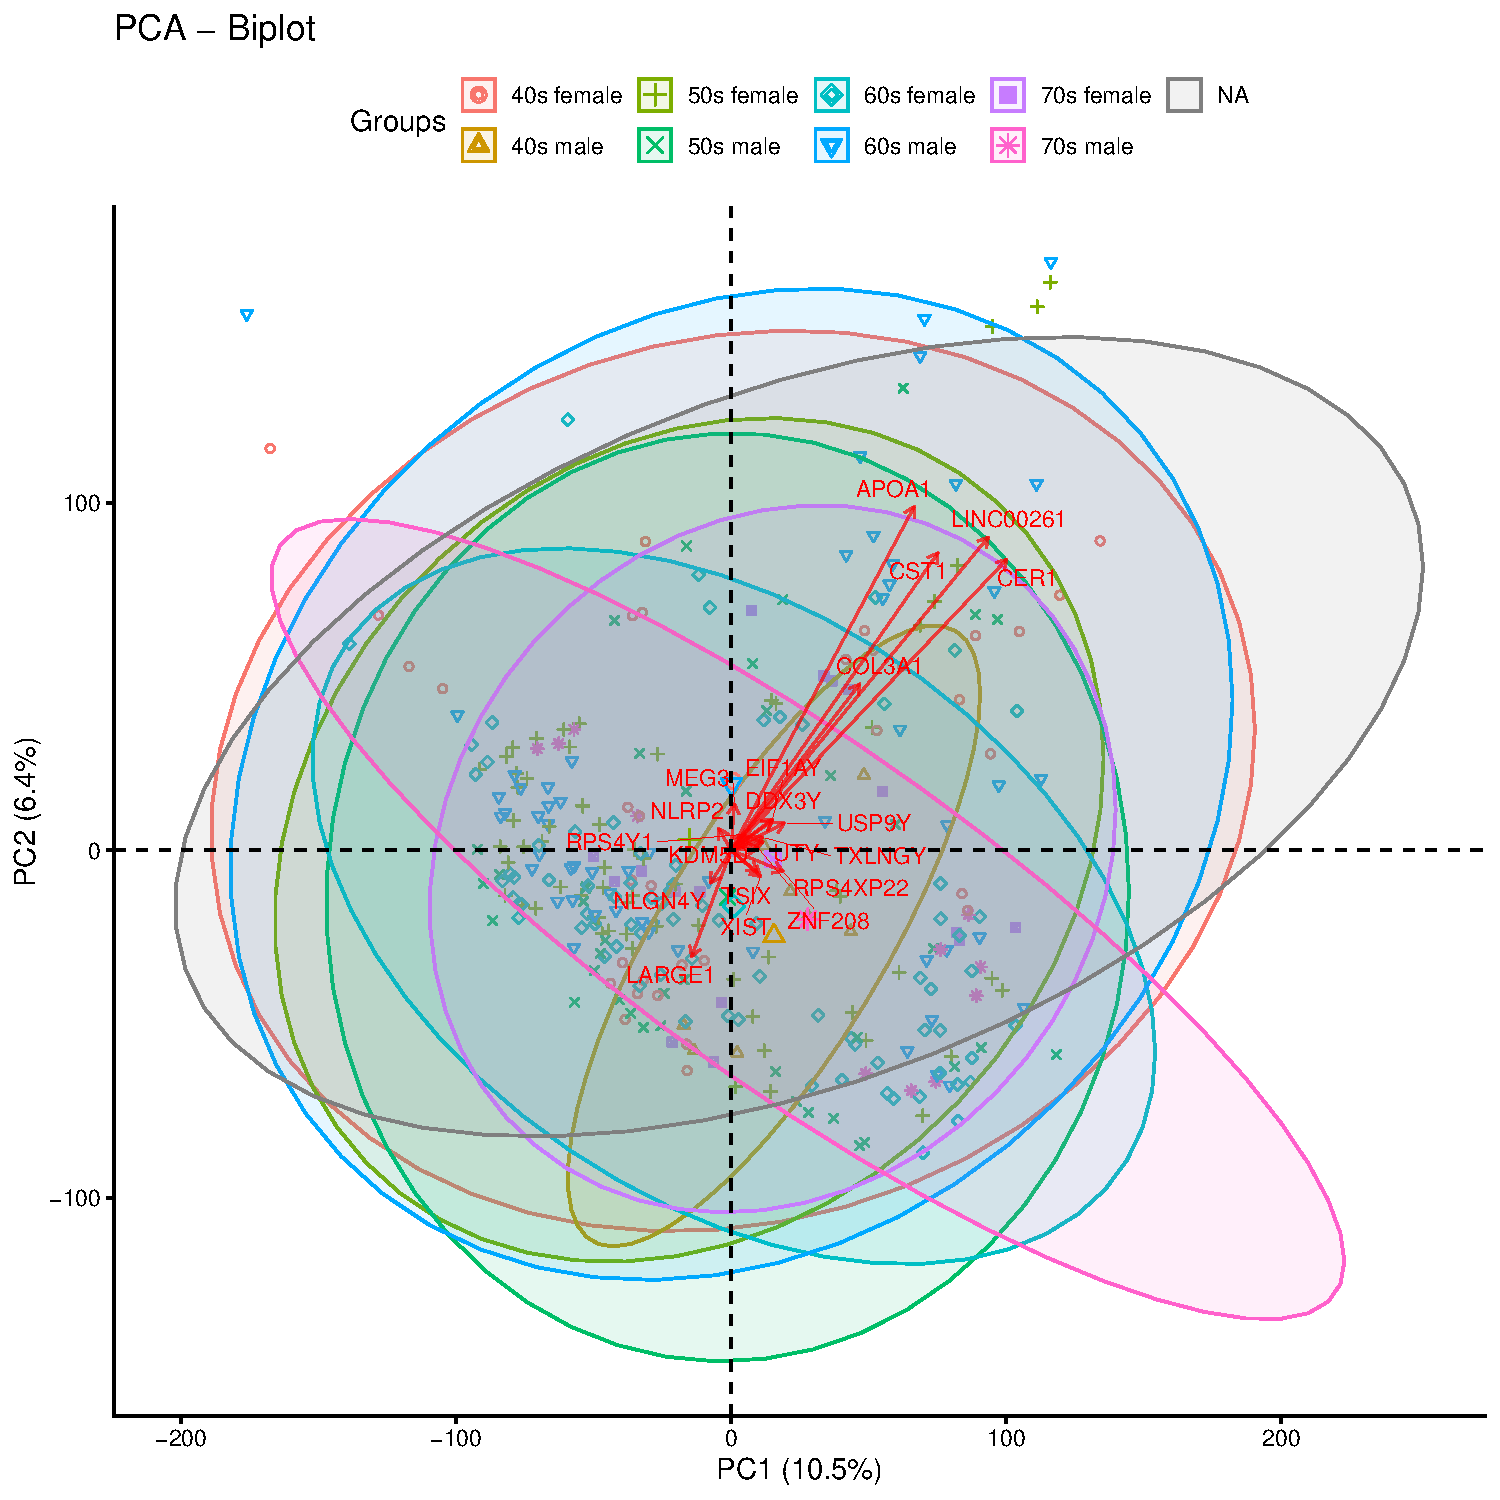
\includegraphics[keepaspectratio]{Final-Project-BIOL806-V4_files/figure-pdf/fig-pca-sexage-1.pdf}}

}

\caption{\label{fig-pca-sexage}Principal Component Analysis (PCA)
grouped by Donor's Age and Sex. PCA of log2 gene expression across all
samples. PCA1 and PCA2 explain 10.5\% and 6.4\# of the variance,
respectively. Sample are colored by age-sex groups and ellipses
represent 95\% confidence intervals for each group. Two twenty genes
contributing most to the variance are labeled as vactors.}

\end{figure}%

\begin{figure}

\centering{

\pandocbounded{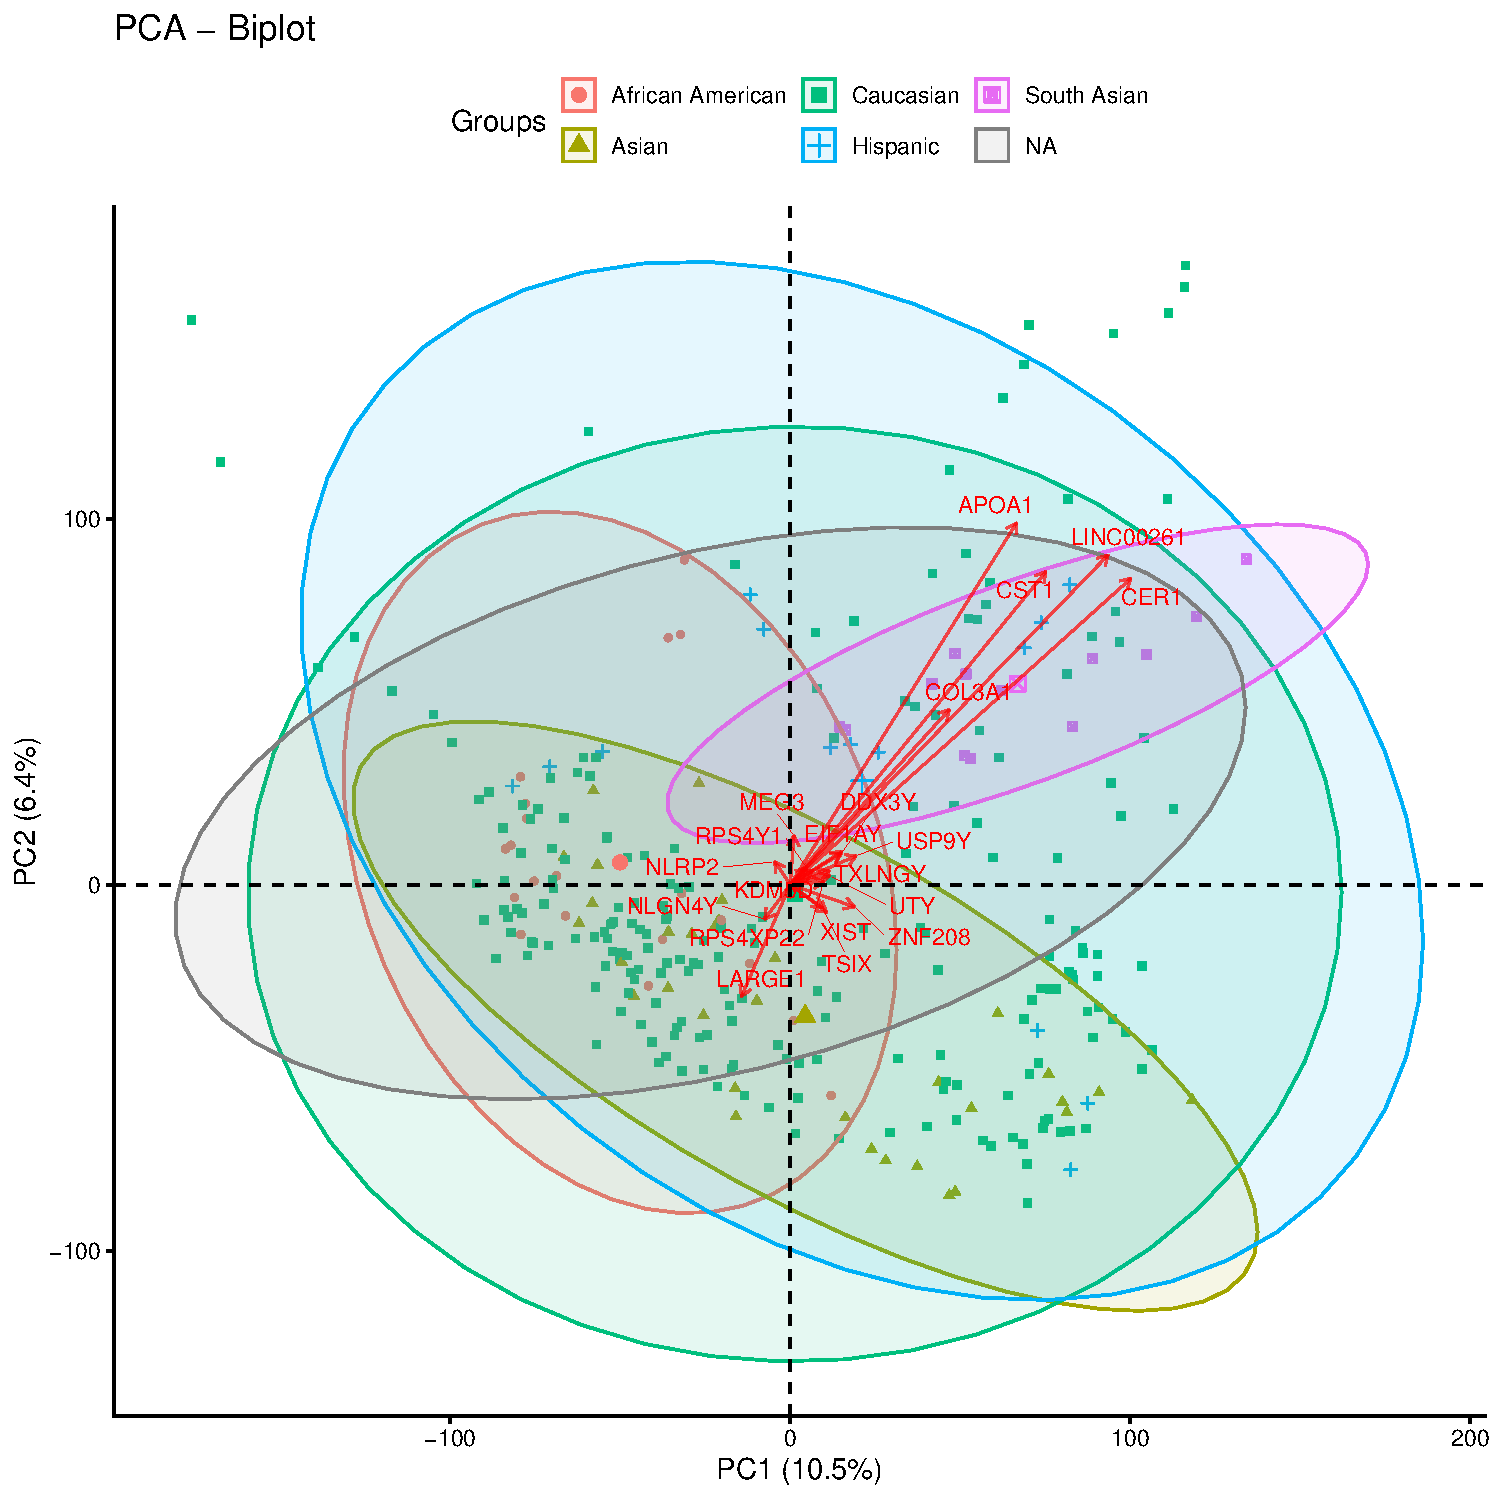
\includegraphics[keepaspectratio]{Final-Project-BIOL806-V4_files/figure-pdf/fig-pca-race-1.pdf}}

}

\caption{\label{fig-pca-race}Principal Component Analysis (PCA) grouped
by Donor's Race. PCA of log2 gene expression across all samples. PCA1
and PCA2 explain 10.5\% and 6.4\# of the variance, respectively. Sample
are colored by race groups and ellipses represent 95\% confidence
intervals for each group. Two twenty genes contributing most to the
variance are labeled as vactors.}

\end{figure}%

\begin{figure}

\centering{

\pandocbounded{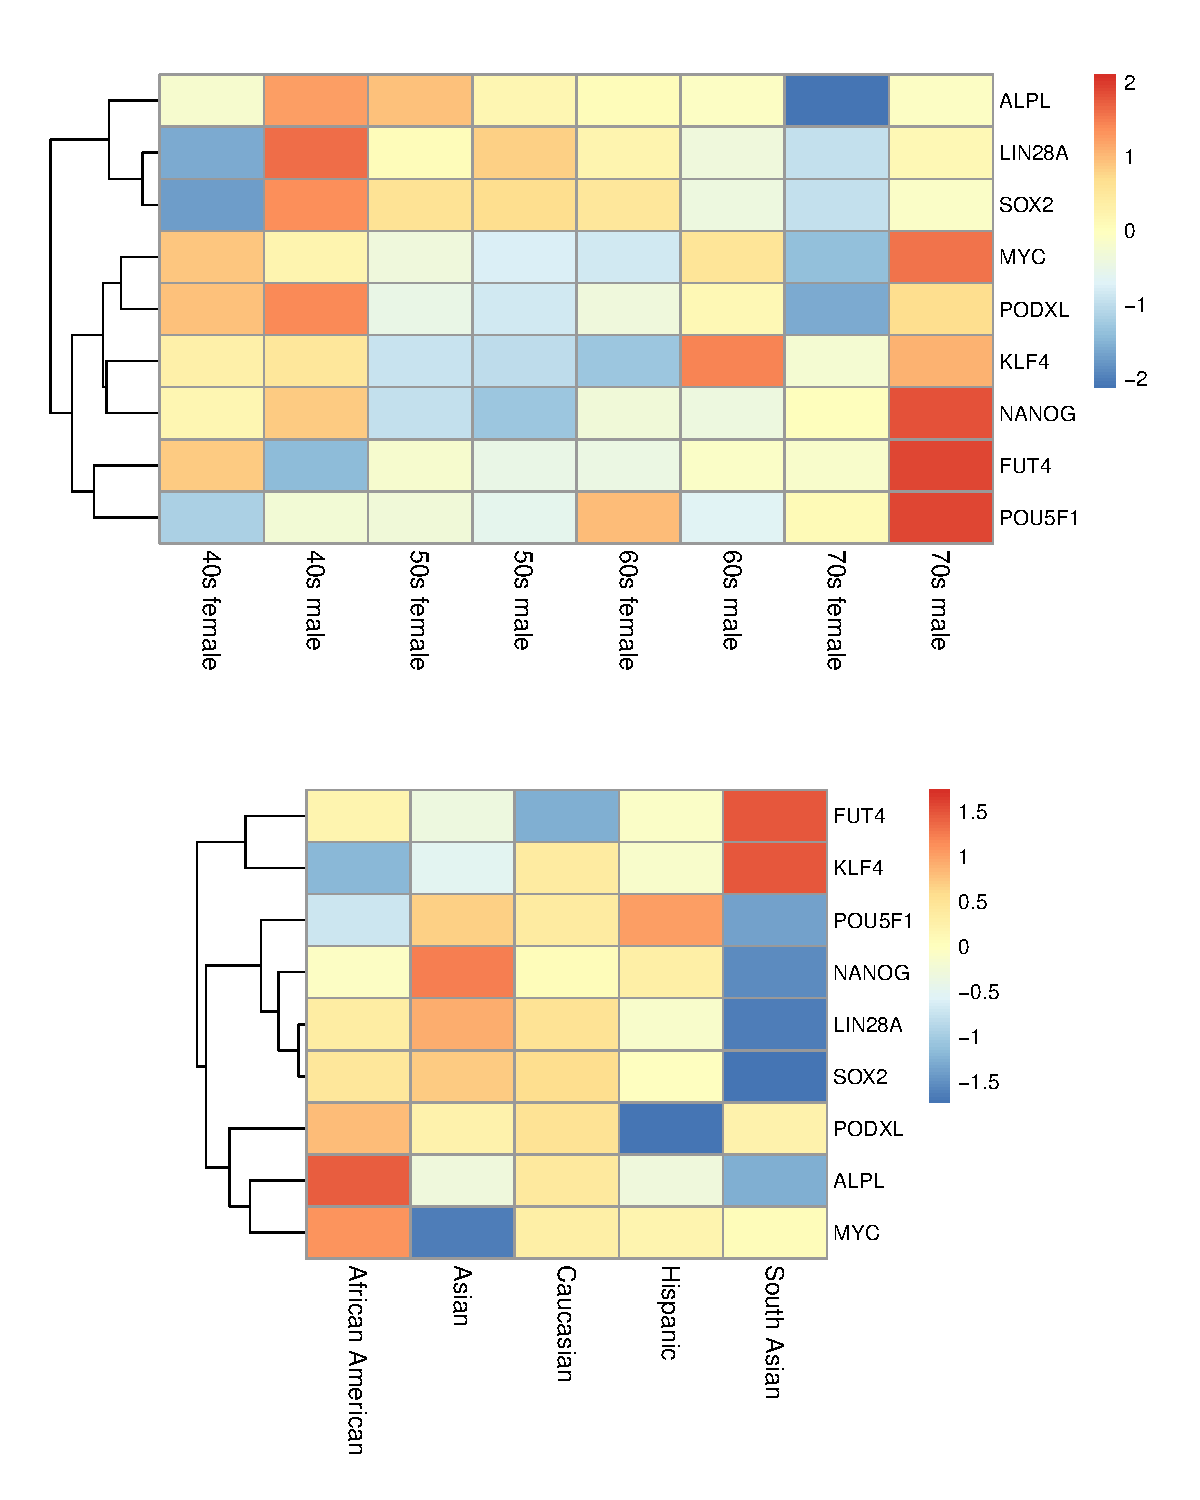
\includegraphics[keepaspectratio]{Final-Project-BIOL806-V4_files/figure-pdf/fig-heatmap-pluripotency-1.pdf}}

}

\caption{\label{fig-heatmap-pluripotency}Heatmap of Pluripotency Gene
Expression. Rows correspond to genes and columns correspond to samples
grouped by age-sex (top) and race (bottom).Colors indicate relative
expression levels based on log2 count per million expression.
Hierarchical clustering was applied to the genes to highlight patterns
of expression.}

\end{figure}%

\begin{figure}

\centering{

\pandocbounded{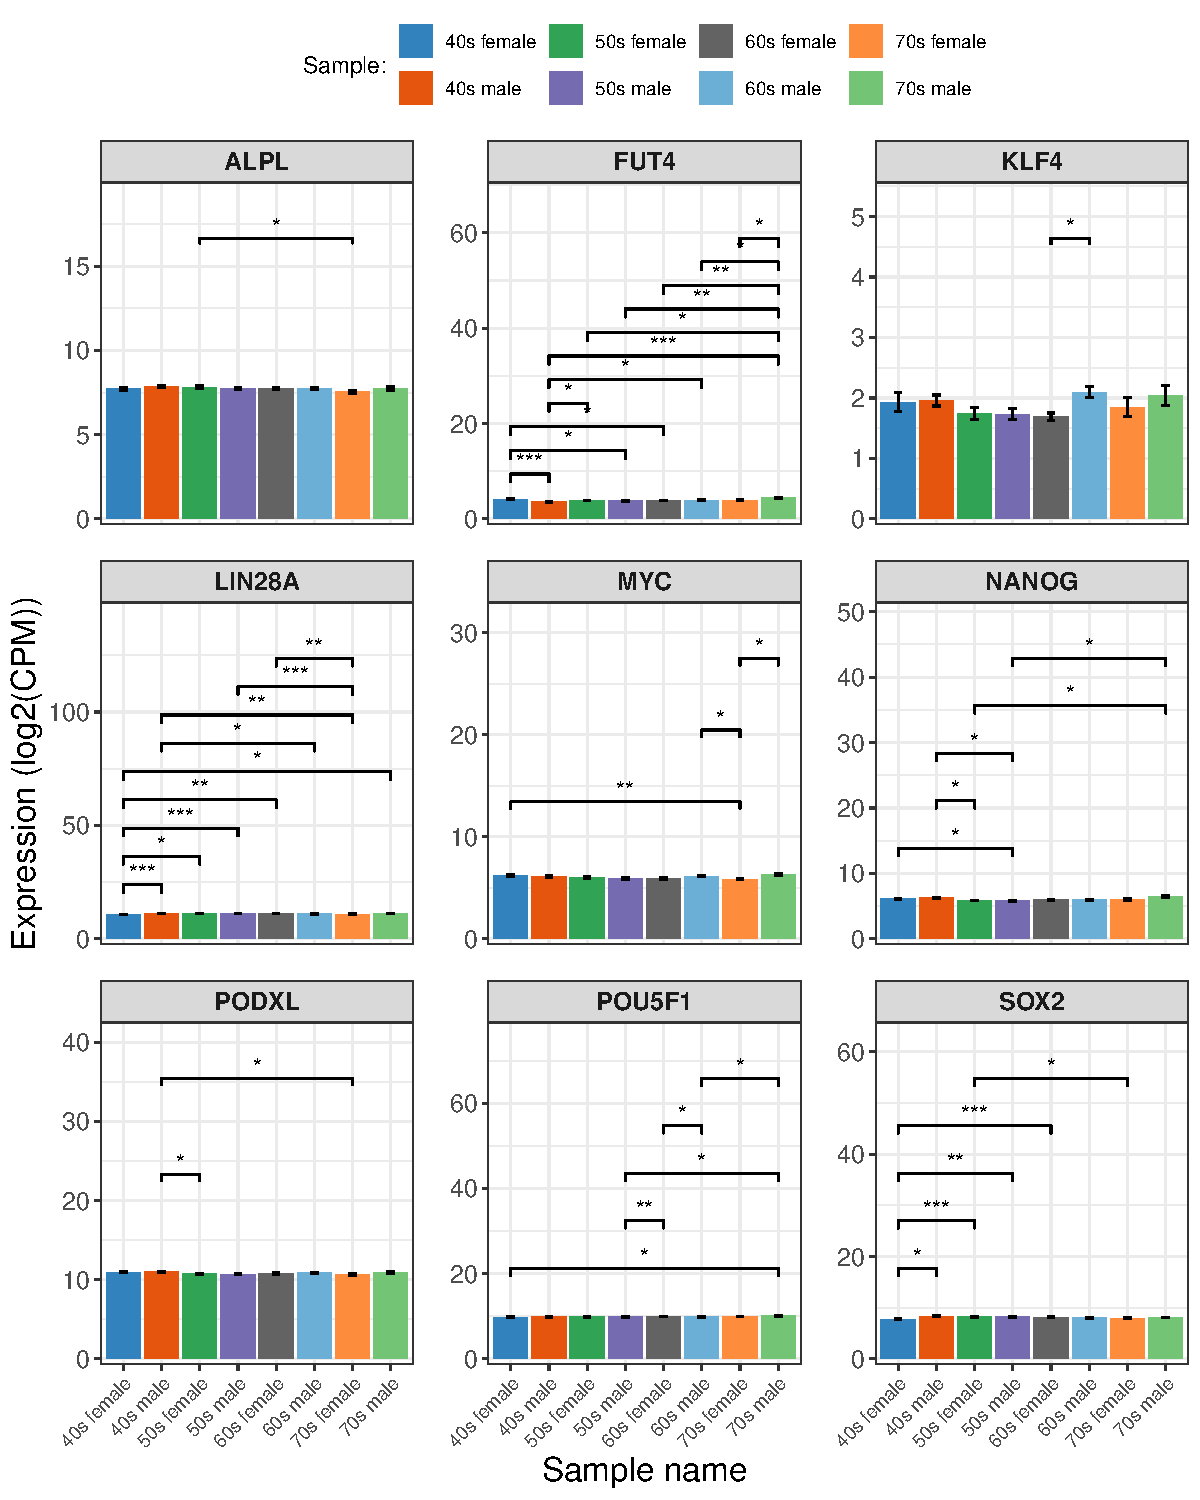
\includegraphics[keepaspectratio]{Final-Project-BIOL806-V4_files/figure-pdf/fig-bargraph-pluripotency-1.pdf}}

}

\caption{\label{fig-bargraph-pluripotency}Expression of Pluripotency
Genes by Age-Sex. Bar plots of log2 count per million gene expression by
pluripotency gene. Bars represent mean expression ± standard error.
Pairwise statistical significance was determined using Games-Howell post
hoc tests following Welch's ANOVA, and significance was indicated with
asterisks: p \textless{} 0.05 (\texttt{*}), p \textless{} 0.01
(\texttt{**}), p \textless{} 0.001 (\texttt{***}).}

\end{figure}%

\begin{figure}

\centering{

\pandocbounded{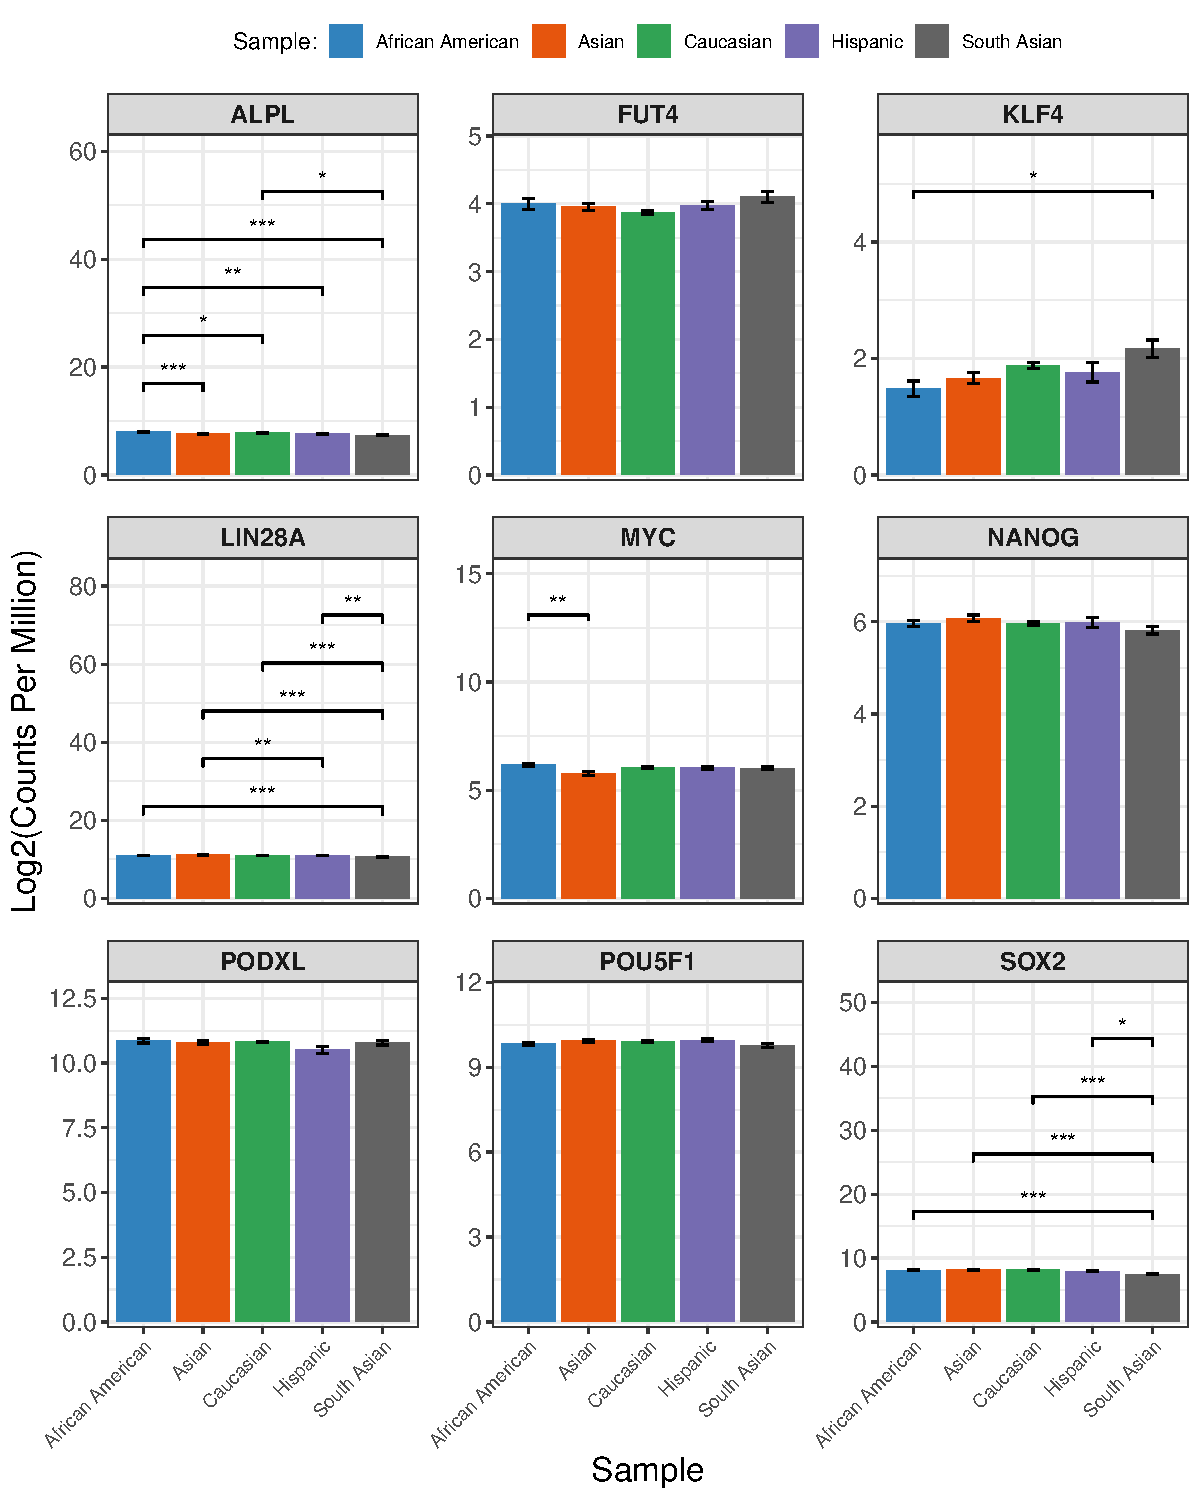
\includegraphics[keepaspectratio]{Final-Project-BIOL806-V4_files/figure-pdf/fig-bargraph-pluripotency-race-1.pdf}}

}

\caption{\label{fig-bargraph-pluripotency-race}Expression of
Pluripotency Genes by Race. Bar plots of log2 count per million gene
expression by pluripotency gene. Bars represent mean expression ±
standard error. Pairwise statistical significance was determined using
Games-Howell post hoc tests following Welch's ANOVA, and significance
was indicated with asterisks: p \textless{} 0.05 (\texttt{*}), p
\textless{} 0.01 (\texttt{**}), p \textless{} 0.001 (\texttt{***})s}

\end{figure}%

\begin{figure}

\centering{

\pandocbounded{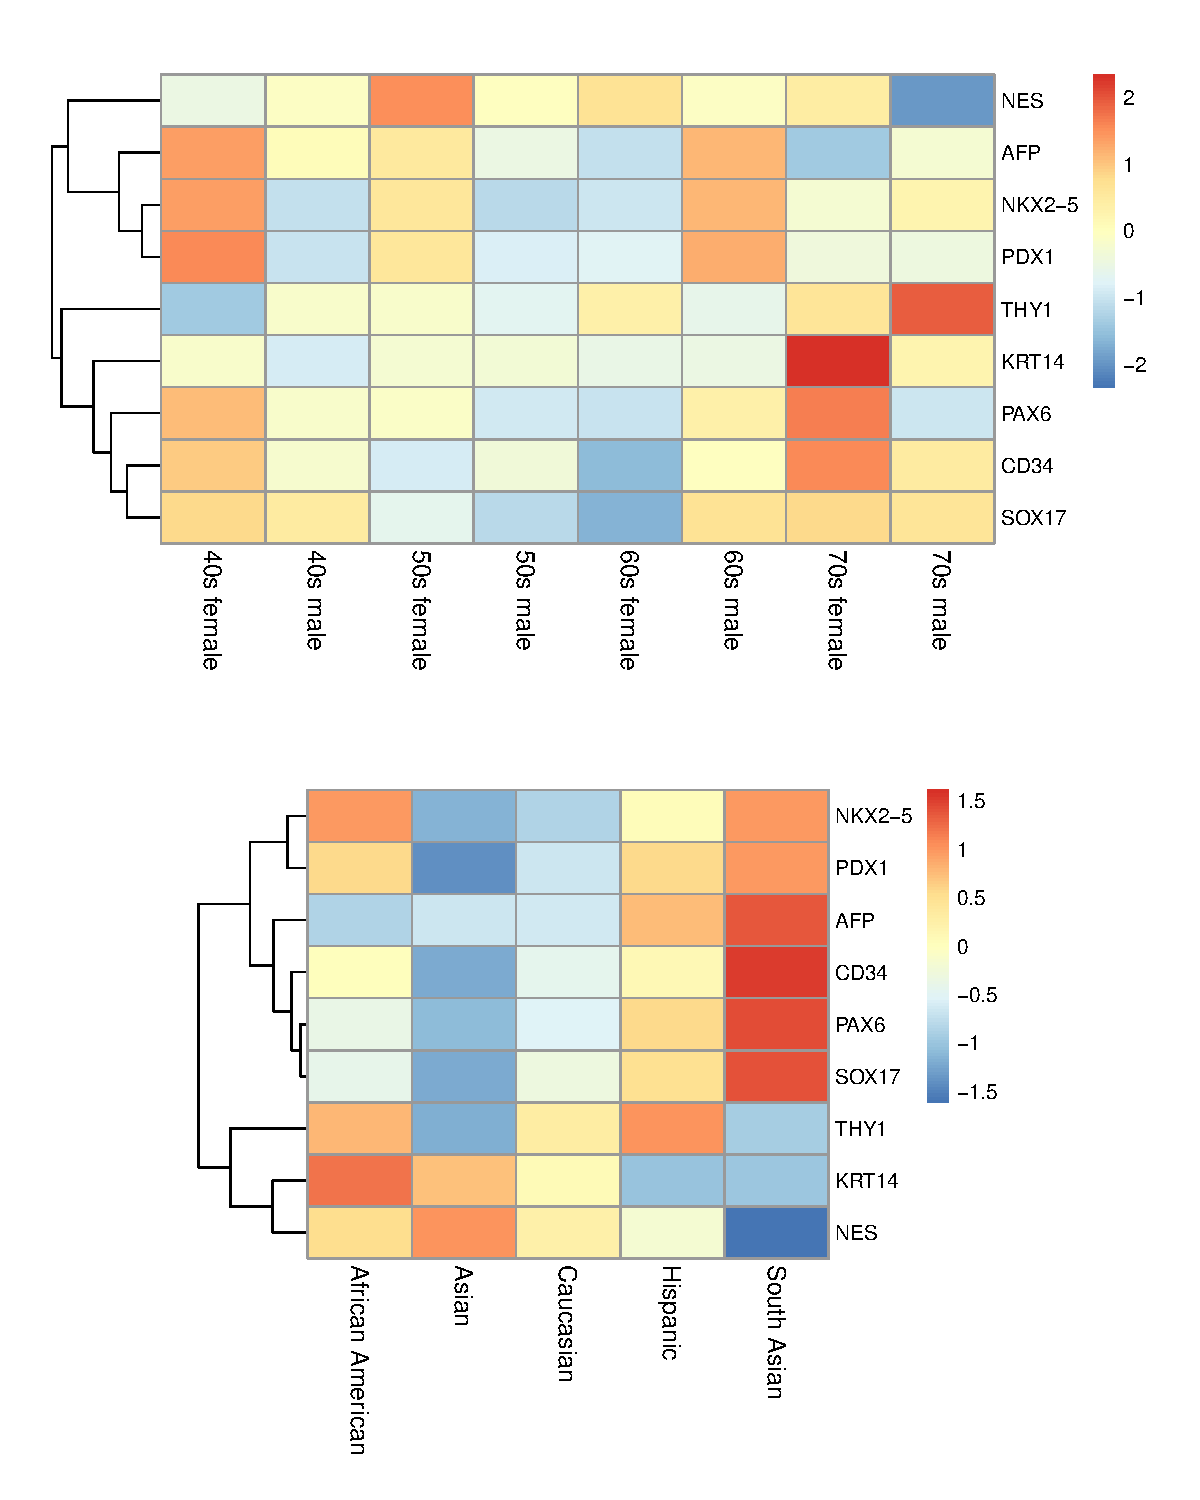
\includegraphics[keepaspectratio]{Final-Project-BIOL806-V4_files/figure-pdf/fig-heatmap-diff-1.pdf}}

}

\caption{\label{fig-heatmap-diff}Heatmap of Differentiation Gene
Expression. Rows correspond to genes and columns correspond to samples
grouped by age-sex (top) and race (bottom).Colors indicate relative
expression levels based on log2 count per million expression.
Hierarchical clustering was applied to the genes to highlight patterns
of expression.}

\end{figure}%

\begin{figure}

\centering{

\pandocbounded{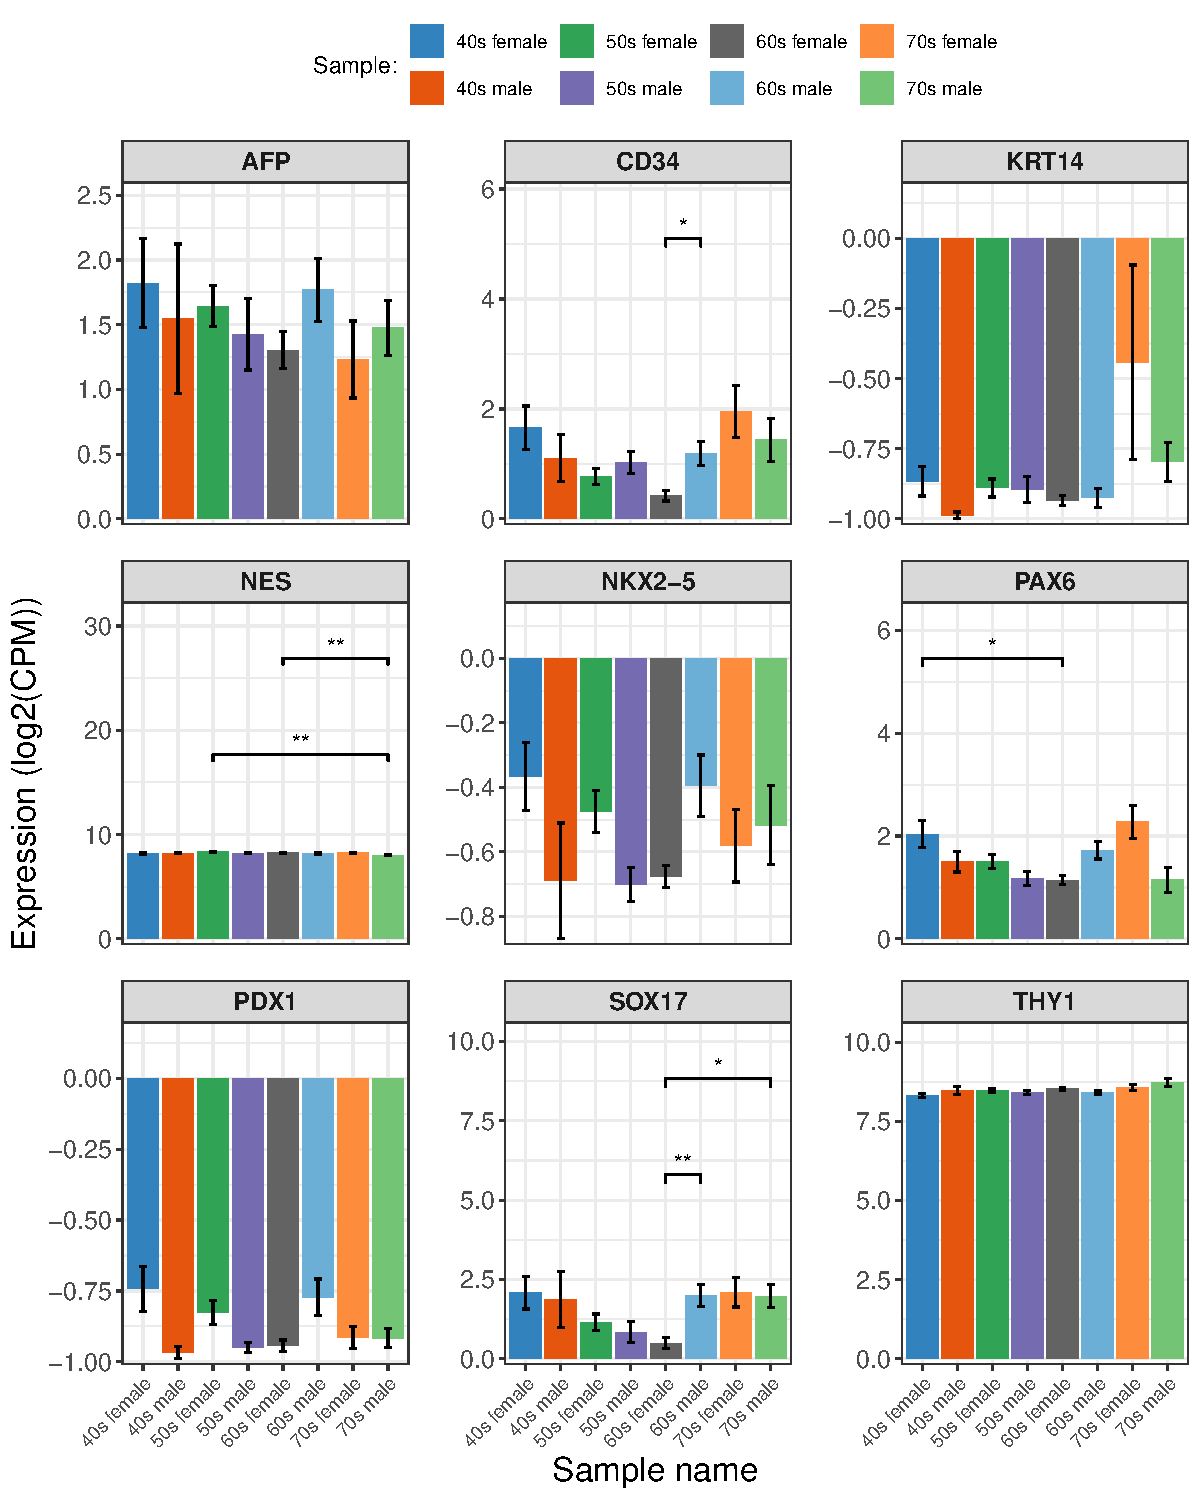
\includegraphics[keepaspectratio]{Final-Project-BIOL806-V4_files/figure-pdf/fig-bargraph-diff-1.pdf}}

}

\caption{\label{fig-bargraph-diff}Expression of Differentiation Genes by
Age-Sex. Bar plots display log2 count per million gene expression by
differentiation gene. Bars represent mean expression ± standard error.
Pairwise statistical significance was determined using Games-Howell post
hoc tests following Welch's ANOVA, and significance was indicated with
asterisks: p \textless{} 0.05 (\texttt{*}), p \textless{} 0.01
(\texttt{**}), p \textless{} 0.001 (\texttt{***}).}

\end{figure}%

\begin{figure}

\centering{

\pandocbounded{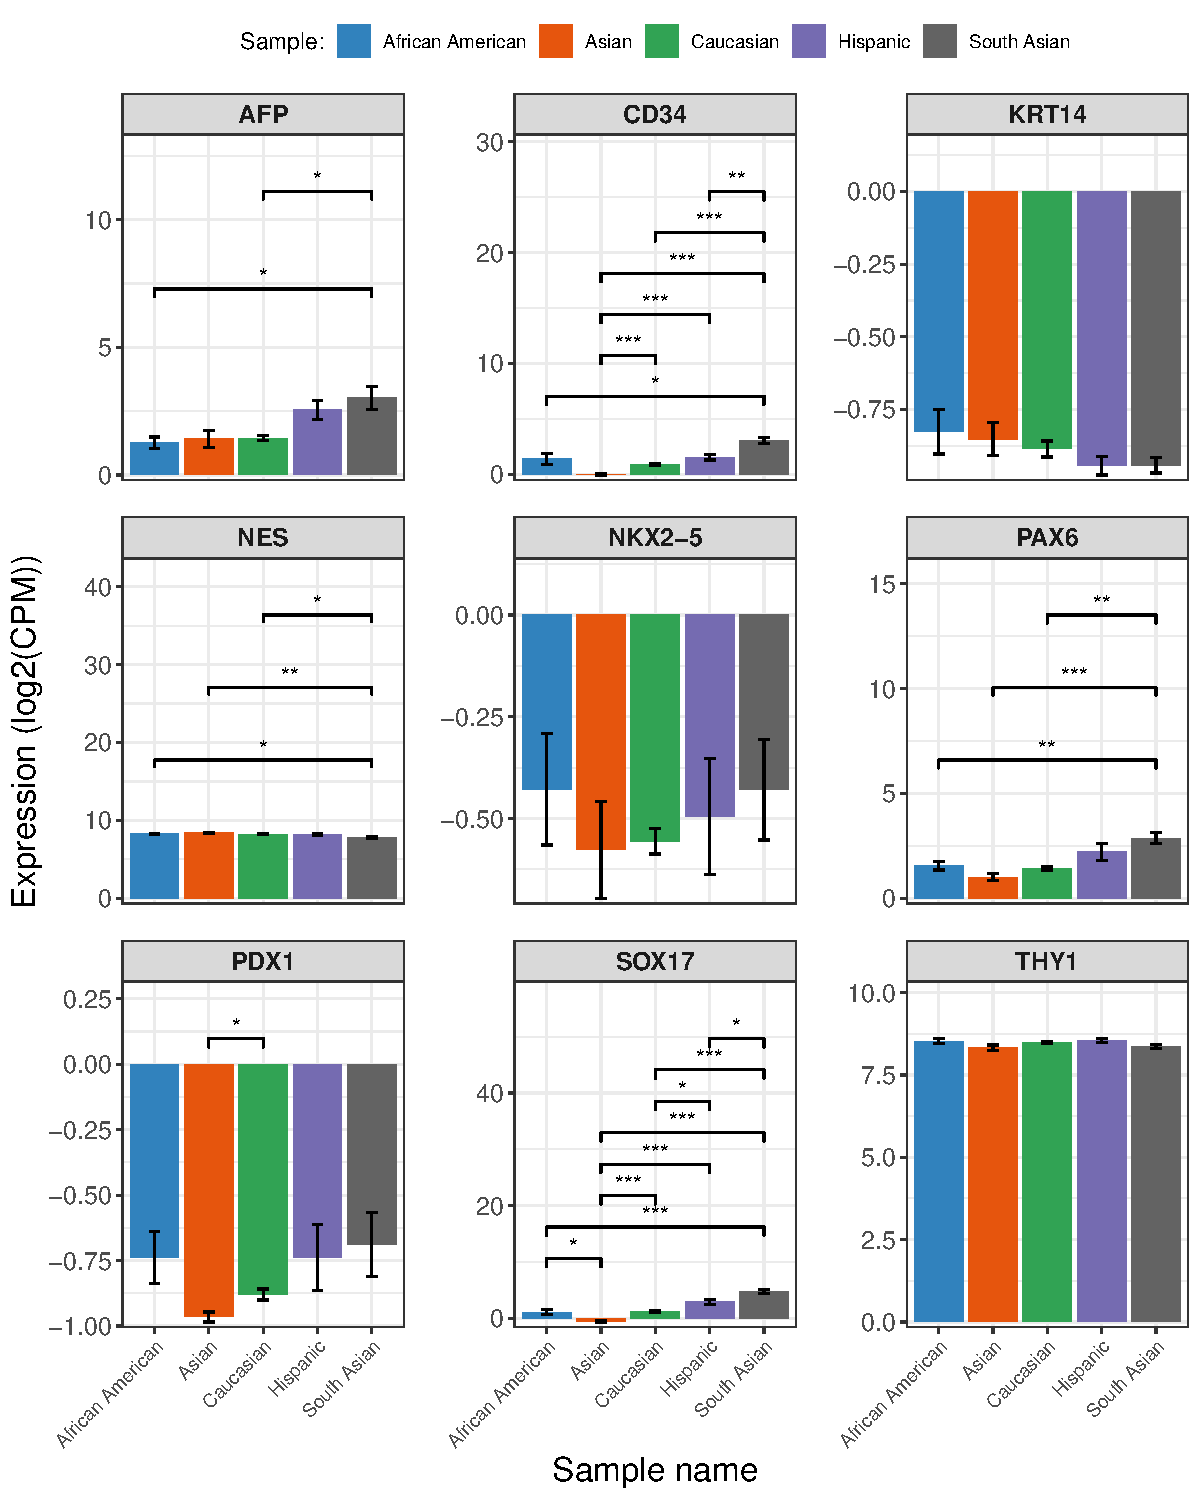
\includegraphics[keepaspectratio]{Final-Project-BIOL806-V4_files/figure-pdf/fig-bargraph-diff-race-1.pdf}}

}

\caption{\label{fig-bargraph-diff-race}Expression of Differentiation
Genes by Race. Bar plots display log2 count per million gene expression
by differentiation gene. Bars represent mean expression ± standard
error. Pairwise statistical significance was determined using
Games-Howell post hoc tests following Welch's ANOVA, and significance
was indicated with asterisks: p \textless{} 0.05 (\texttt{*}), p
\textless{} 0.01 (\texttt{**}), p \textless{} 0.001 (\texttt{***}).}

\end{figure}%

\begin{figure}

\centering{

\pandocbounded{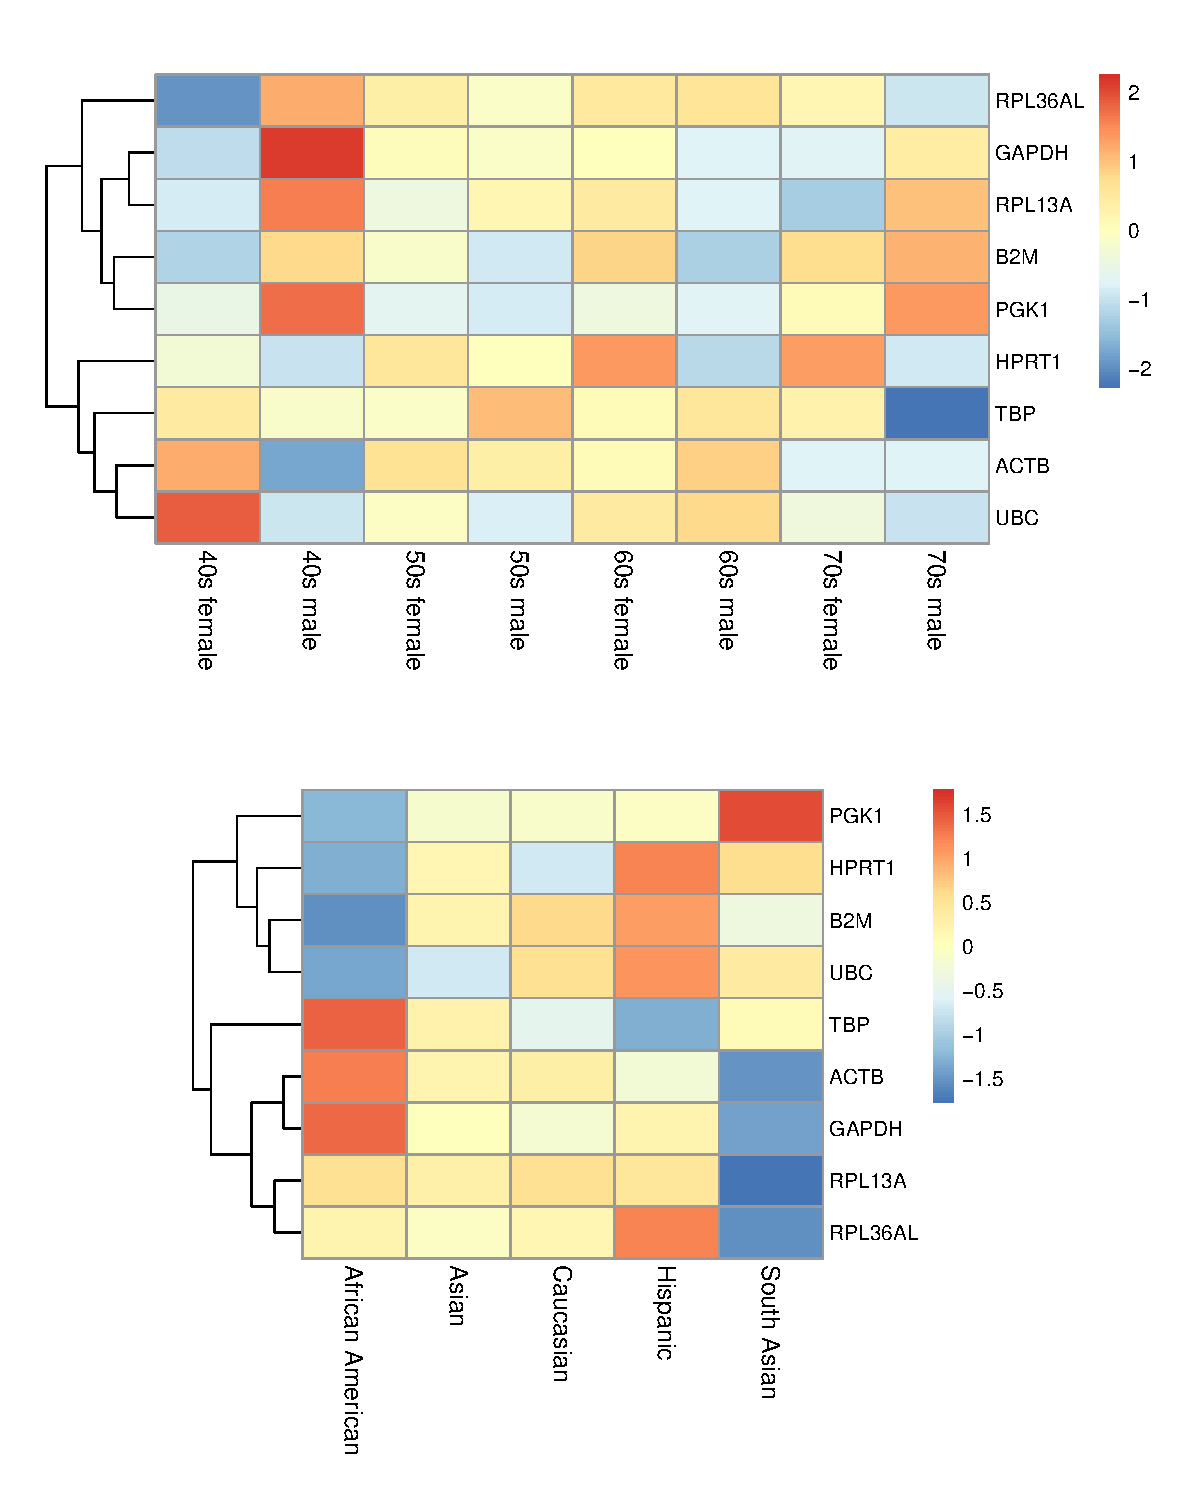
\includegraphics[keepaspectratio]{Final-Project-BIOL806-V4_files/figure-pdf/fig-heatmap-hk-1.pdf}}

}

\caption{\label{fig-heatmap-hk}Heatmap of Housekeeping Gene Expression.
Rows correspond to genes and columns correspond to samples grouped by
age-sex (top) and race (bottom).Colors indicate relative expression
levels based on log2 count per million expression. Hierarchical
clustering was applied to the genes to highlight patterns of
expression.}

\end{figure}%

\begin{figure}

\centering{

\pandocbounded{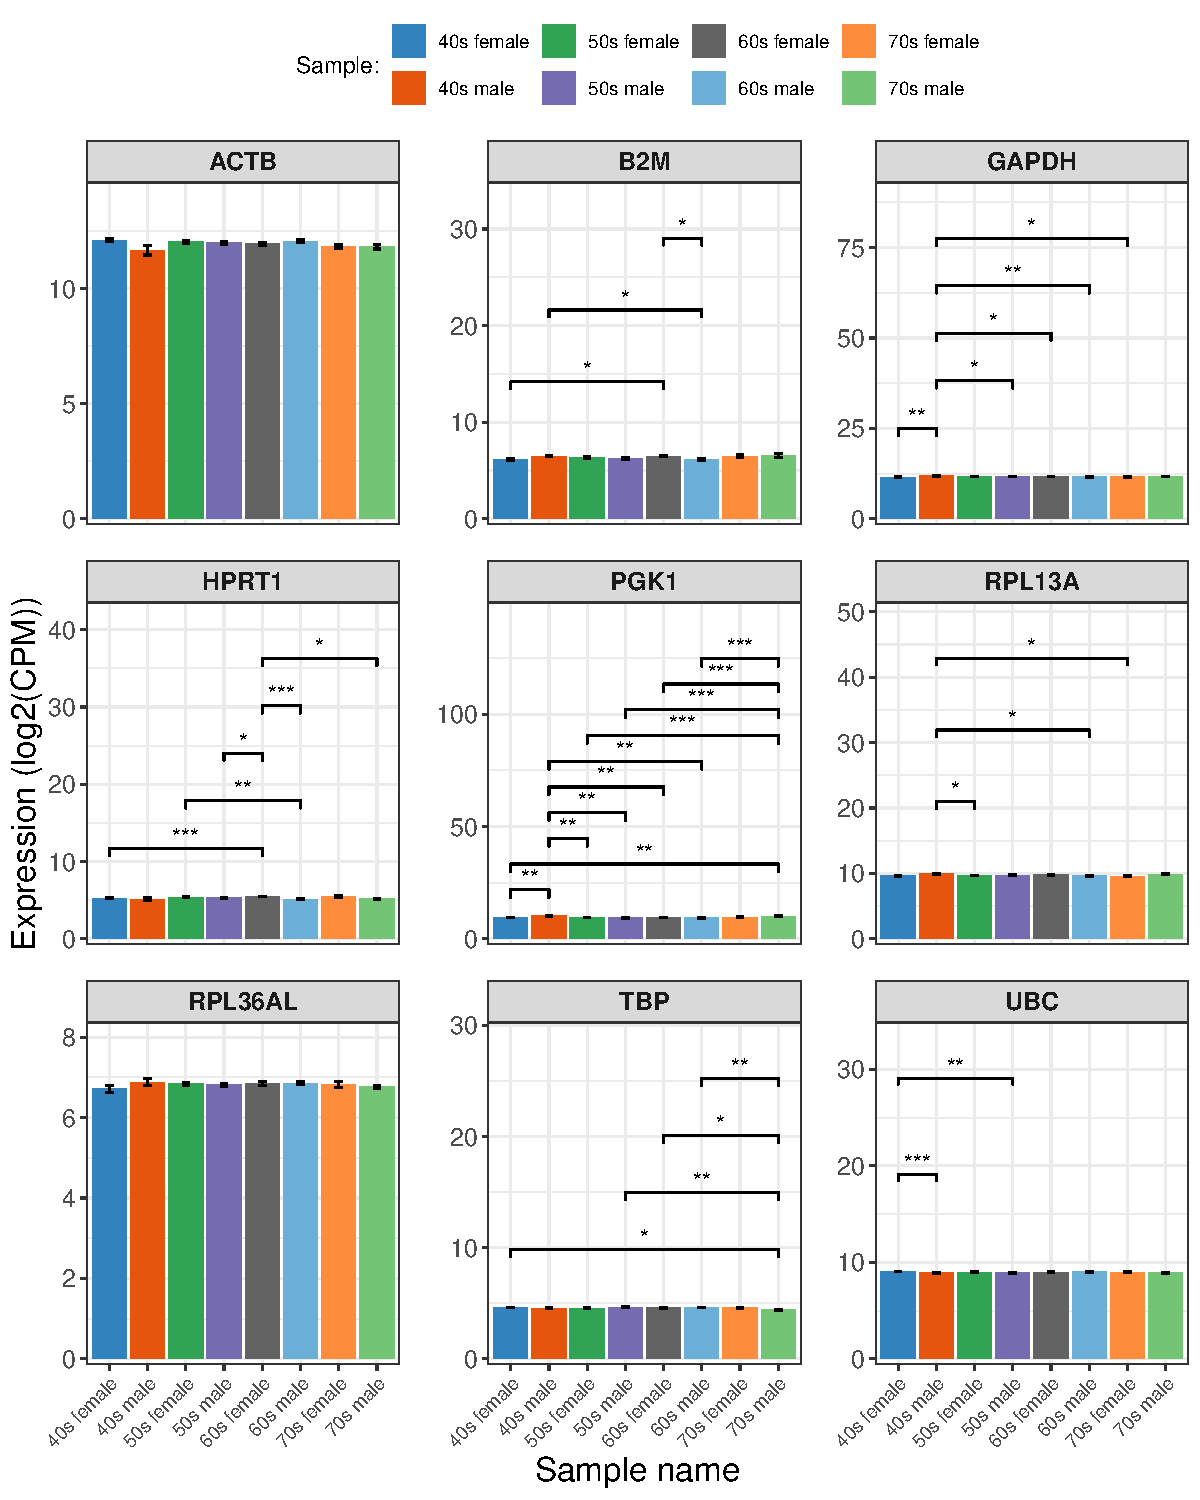
\includegraphics[keepaspectratio]{Final-Project-BIOL806-V4_files/figure-pdf/fig-bargraph-hk-1.pdf}}

}

\caption{\label{fig-bargraph-hk}Expression of Housekeeping Genes by
Age-Sex. Bar plots display log2 count per million gene expression by
housekeeping gene. Bars represent mean expression ± standard error.
Pairwise statistical significance was determined using Games-Howell post
hoc tests following Welch's ANOVA, and significance was indicated with
asterisks: p \textless{} 0.05 (\texttt{*}), p \textless{} 0.01
(\texttt{**}), p \textless{} 0.001 (\texttt{***}).}

\end{figure}%

\begin{figure}

\centering{

\pandocbounded{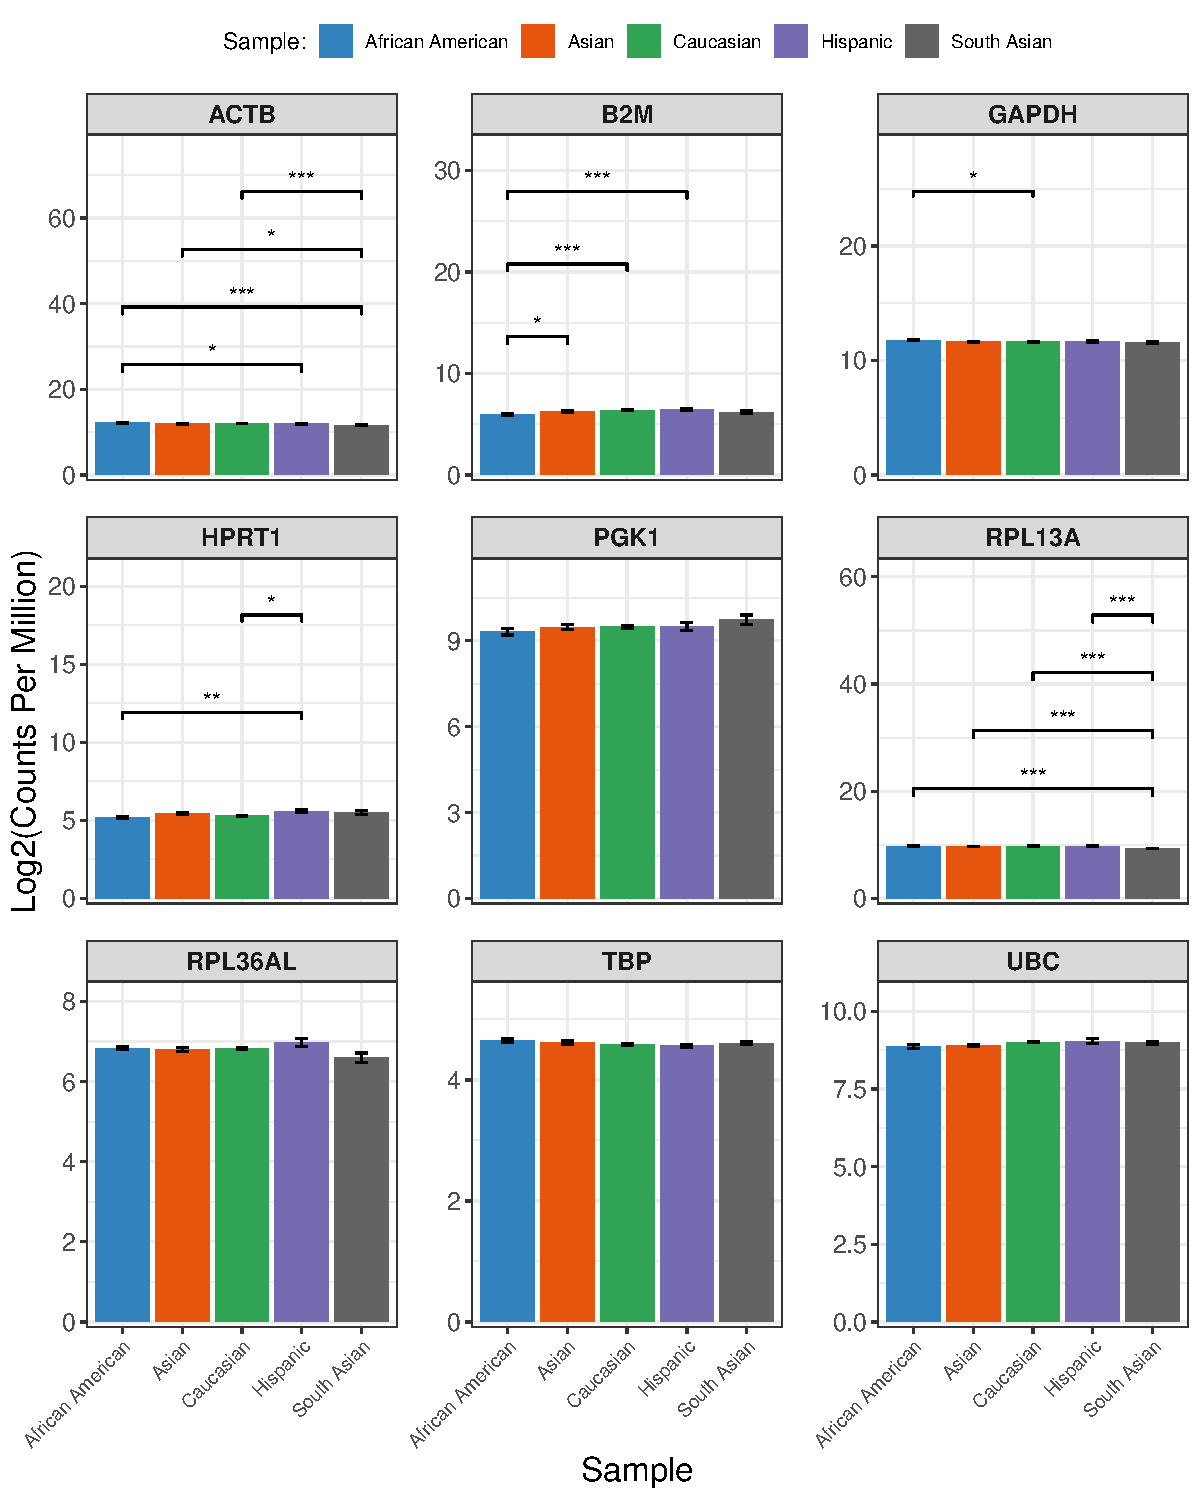
\includegraphics[keepaspectratio]{Final-Project-BIOL806-V4_files/figure-pdf/fig-bargraph-hk-race-1.pdf}}

}

\caption{\label{fig-bargraph-hk-race}Expression of Housekeeping Genes by
Race. Bar plots display log2 count per million gene expression by
housekeeping gene. Bars represent mean expression ± standard error.
Pairwise statistical significance was determined using Games-Howell post
hoc tests following Welch's ANOVA, and significance was indicated with
asterisks: p \textless{} 0.05 (\texttt{*}), p \textless{} 0.01
(\texttt{**}), p \textless{} 0.001 (\texttt{***}).}

\end{figure}%

\section{Discussion}\label{discussion}

\subsubsection{pie charts}\label{pie-charts}

The RNA Seq data is composed of a variety of different types of RNA, as
seen in Figure 1. 34.8\% of read genes are mRNA protein coding genes,
whereas the remaining 65.2\% of the detected genes are not protein
coding and are primary composed of noncoding RNAs and pseudogenes, which
are RNA sequences that look like protein coding genes but are not able
to be translated into a protein. 25.6\% of the detected genes were
pseuodegenes. 25.5\% were long non coding RNA sequences and 8.5\% were
small RNAs, which included snoRNA, snRNA, scaRNA, sRNA, and ribozyme
RNA. 5.7\% were ``Other'' RNAs, which include ribosoal RNA, immunoglobin
genes, T-cell receptor genes, and mitocondrial RNAs. The right pie
chart, on the other hand, displays the expression of these groups. For
each gene for each sample, a count per million number was provided by
Carcamo-Orive \emph{et al.}. This is typically calculated by dividing
the raw count of the gene by the total reads in the sample and
multiplying by one million. The total expression was summed for each
category, and this was graphed in Figure 2, which displays that 91.7\%
of the expression is from protein coding genes. The remaining 8.3\%
accounts for the expression of small RNAs, long non coding RNA,
pseuodgenes, and ``Other'' genes. This is supported by \_\_\_ data from
\_\_\_ article, which saw \_\_\_\_.

\subsubsection{pca}\label{pca}

welch's anova (one way analysis of means (not assuming equal variance)

PC1 and sex (p = 0.3892) PCA2 ( p = 0.6077)

PCA1 and age\_Decade (p = 0.09443) and PCA2 (p = 0.2645)

PCA1 and age\_sex (p = 0.1993) and PCA2 (p \textless{} 0.001)

PCA1 and race (p \textless{} 0.001) and PCA2 (p \textless{} 0.001)

When tested independently, neither age nor sex was significantly
associated with PC1 or PC2.\\

However, when individuals were grouped by age--sex categories, a
significant effect emerged (Welch's ANOVA p = ), suggesting that
specific combinations of age and sex capture multivariate expression
patterns not explained by either variable alone.

\subsubsection{top 20 genes:}\label{top-20-genes}

sex linked RPS4Y1 Ribosomal protein S4, Y-linked. Present only in males.
High variance indicates sex is a strong driver. XIST X-inactive specific
transcript. Expressed in females for X-chromosome inactivation.
Sex-linked. DDX3Y DEAD-box helicase, Y-linked. Male-specific. TSIX
Antisense of XIST, regulates X-chromosome inactivation. Female-specific.
TXLNGY Y-linked, involved in transcription/translation regulation. KDM5D
Lysine demethylase 5D, Y-linked. Male-specific. USP9Y Ubiquitin-specific
peptidase 9, Y-linked. Male-specific. EIF1AY Eukaryotic translation
initiation factor 1A, Y-linked. Male-specific. UTY Ubiquitously
transcribed tetratricopeptide repeat, Y-linked. Male-specific. NLGN4Y
Neuroligin 4, Y-linked. Male-specific. RPS4XP22 Pseudogene similar to
RPS4X/RPS4Y.

other genes CST1 Cystatin SN, extracellular protease inhibitor. May vary
in differentiation. CER1 Cerberus, secreted factor involved in early
development and differentiation. LARGE1 Glycosyltransferase, involved in
post-translational modification. NLRP2 NLR family pyrin domain
containing 2, involved in early development, oocyte/embryo regulation.
COL3A1 Collagen type III alpha 1, ECM protein, differentiation-related.
ZNF208 Zinc finger protein, transcription factor, potential regulatory
role. APOA1 Apolipoprotein A1, lipid transport, may reflect metabolic
differences. MEG3 Long non-coding RNA, tumor suppressor, epigenetic
regulation, differentiation-related. LINC00261 Long non-coding RNA,
involved in endoderm differentiation.

\subsubsection{Pluripotency, Differentiation, and Houskeeping Gene
Expression}\label{pluripotency-differentiation-and-houskeeping-gene-expression}

The expression of pluripotency genes, SOX2, OCT4 (POU5F1), KLF4, c-Myc
(MYC), TRA-1-81 and 1-60 (PODXL), NANOG, SSEA4 (FUT4), LIN28A, and
Alkaline Phosphatase (ALPL)., were analyzed after grouping by both
age-sex and race. These genes include transcription factors, SOX2, OCT4,
KLF4, and NANOG, involved in maintaining a pluripotent state, cell
surface markers, SSEA4 and TRA-1-81/TRA-1-60, RNA binding protein,
LIN28A, and a highly expressed enzyme in pluripotent cells, Alkaline
Phosphatase. These genes have been found to be highly expressed in
pluripotent cells, such as iPSCs., (\_\_\_\_\_\_source).

To determine if the expression of these pluripotent genes varied across
conditions, two linear mixed models were used. Expression was modeled as
a function of age-sex, with random intercepts grouped by gene to account
for baseline differences in gene expression, where j represents the
observation of each gene, i, and u represents the part of the intercept
that is unique to each gene.

\[
\hat{Expression}_{ij} = \beta_0 + \beta_1 ({age\_sex}_{ij}) + u_{0j} + \varepsilon_{ij}
\]

The same model was then run, but using race as the fixed effect. In both
cases, Type III Analysis of Variance Table with Satterthwaite's method
were used to determine which groups had statically significance
differences in gene expression when compared to the reference groups
(female 40s and African American).

Residual variance was 0.189 and 0.190 when grouping by age-sex and race,
respectively, and gene intercept variance was 9.82 for both. This
suggests that the majoirty of the variance is between genes, not between
groups. It was found that 70s female group displayed a 6.5\% decrease in
pluripotency expression ( - 0.097, p \textless{} 0.05.), whereas 70s
male saw a 13\% increase in pluripotency expression (+0.179, p
\textless{} 0.001).

no difference between other groups and the reference group (40s female)

Type III Analysis of Variance Table with Satterthwaite's method -
confirms age\_sex have a significant effect on pluripotency gene
expression when averaged across all genes. p \textless{} 0.001.

FUT4 showed 11 significant pairwise comparisons across age-sex groups
after FDR correction (Games-Howell test), LIN28A showed 9, and NANOG,
POU5F1, and SOX2 with 5 signficant pairwiese comparisons.

KLF4 and ALPL showed the fewest significant differences, with only one
pairwise comparison reaching significance.

all gene has significant pairwise comparisons

linear mixed model Expression \textasciitilde{} race +
1\textbar{}\texttt{Gene\ name}

Residual variance = 0.1901 and gene intercept variance = 9.82 means most
of the variation is between genes, not race. the genes differ a lot.
residual noise is small, model fits wells

South Asian 2\^{}(-0.143) = 0.9 = 10\% decrease in expression. (p
\textless{} 0.01)

After adjusting for gene-level random effects, South Asian individuals
show significantly lower mean log₂ gene expression (β = --0.143, p =
0.0059).\\

This corresponds to approximately a 10\% decrease in pluripotency gene
expression relative to the reference race group.

ALPL and LIN28A showed 5 significant pairwise comparisons, and SOX2 with
four.

Several pluripotency genes, including FUT4, NANOG, PODXL, and POU5F1,
did not show any significant pairwise differences across age-sex groups,
indicating relatively stable expression.

\subsubsection{Differentiation Markers}\label{differentiation-markers}

Expression of Differentiation Genes (ectoderm: PAX6, NESTIN (NES)
(neural projenitor/stem cell markers), KRT14 (epithelial), endoderm:
SOX17, AFP (hepatic), PDX1 (pancreatic), mesoderm: CD34 (hematopoitic),
CD90 (THY1)(mesenchymal), NKX2.5 (cardiac progenitor)).

age\_sex

random effects:

Gene-level intercept variance = 13.168 (SD = 3.629), showing substantial
variation between genes.

Residual variance = 1.195 (SD = 1.093), within-gene variation.

fixed effects

50s female, -0.269, p \textless{} 0.001 17\% decrease

50s male -0.398, p\textless{} 0.001 24.5\% decrease

60s female -0.500, p \textless{} 0.001 29.3\% decrease

Compared with 40s female samples, differentiation gene expression was
17\% lower in 50s female, 24.5\% lower in 50s male, and 29.3\% lower in
60s female samples (p \textless{} 0.001 for all). No significant
differences were observed for 40s male, 60s male, 70s female, or 70s
male.''

race

Intercept 13.169 Residual1.163

Asian, -0.42975, 25.3\% decrease p \textless{} 0.001

Hispanic, + 0.39902, 32.0\% increase, p \textless{} 0.01

South Asian, + 0.85435, 80.0\% increase, p \textless{} 0.001

\subsubsection{Housekeeping Genes}\label{housekeeping-genes}

Figure 5. Expression of Housekeeping Genes (some sort of general figure
or sorted by housekeeping type (i.e.~ribosomal, metabolic, cytoskeleton,
etc.))

age\_sex

Intercept 7.163 Residual 0.150

40s male, + 0.1325, 9.6\% increase, p \textless{} 0.001

50s female, + 0.03375, 2.4\% increase, p \textless{} 0.01

60s female, + 0.08191, 5.7\% increase, p \textless{} 0.01

race

Intercept 7.1635 Residual 0.1507

Hispanic, + 0.09717, 7.1\% increase, p \textless{} 0.05

\section{Conclusion}\label{conclusion}

\begin{center}\rule{0.5\linewidth}{0.5pt}\end{center}

\section*{References}\label{references}
\addcontentsline{toc}{section}{References}

\phantomsection\label{refs}
\begin{CSLReferences}{1}{0}
\bibitem[\citeproctext]{ref-artyukhov2017}
Artyukhov, A. S., Dashinimaev, E. B., Tsvetkov, V. O., Bolshakov, A. P.,
Konovalova, E. V., Kolbaev, S. N., Vorotelyak, E. A. \& Vasiliev, A. V.
(2017). New genes for accurate normalization of qRT-PCR results in study
of iPS and iPS-derived cells. \emph{Gene}, \emph{626}, 234--240.
\url{https://doi.org/10.1016/j.gene.2017.05.045}

\bibitem[\citeproctext]{ref-R-lme4}
Bates, D., Maechler, M., Bolker, B. \& Walker, S. (2025). \emph{lme4:
Linear mixed-effects models using eigen and S4}.
\url{https://github.com/lme4/lme4/}

\bibitem[\citeproctext]{ref-carcamo-orive2017}
Carcamo-Orive, I., Hoffman, G. E., Cundiff, P., Beckmann, N. D.,
D'Souza, S. L., Knowles, J. W., Patel, A., Papatsenko, D., Abbasi, F.,
Reaven, G. M., Whalen, S., Lee, P., Shahbazi, M., Henrion, M. Y. R.,
Zhu, K., Wang, S., Roussos, P., Schadt, E. E., Pandey, G., \ldots{}
Lemischka, I. (2017). Analysis of Transcriptional Variability in a Large
Human iPSC Library Reveals Genetic and Non-genetic Determinants of
Heterogeneity. \emph{Cell Stem Cell}, \emph{20}(4), 518--532.e9.
\url{https://doi.org/10.1016/j.stem.2016.11.005}

\bibitem[\citeproctext]{ref-cerneckis2024}
Cerneckis, J., Cai, H. \& Shi, Y. (2024). Induced pluripotent stem cells
(iPSCs): molecular mechanisms of induction and applications.
\emph{Signal Transduction and Targeted Therapy}, \emph{9}(1), 112.
\url{https://doi.org/10.1038/s41392-024-01809-0}

\bibitem[\citeproctext]{ref-R-FactoMineR}
Husson, F., Josse, J., Le, S. \& Mazet, J. (2025). \emph{FactoMineR:
Multivariate exploratory data analysis and data mining}.
\url{http://factominer.free.fr}

\bibitem[\citeproctext]{ref-R-pheatmap}
Kolde, R. (2025). \emph{Pheatmap: Pretty heatmaps}.
\url{https://doi.org/10.32614/CRAN.package.pheatmap}

\bibitem[\citeproctext]{ref-R-lmerTest}
Kuznetsova, A., Bruun Brockhoff, P. \& Haubo Bojesen Christensen, R.
(2020). \emph{lmerTest: Tests in linear mixed effects models}.
\url{https://github.com/runehaubo/lmerTestR}

\bibitem[\citeproctext]{ref-panina2020}
Panina, Y., Germond, A. \& Watanabe, T. M. (2020). Analysis of the
stability of 70 housekeeping genes during iPS reprogramming.
\emph{Scientific Reports}, \emph{10}, 21711.
\url{https://doi.org/10.1038/s41598-020-78863-5}

\bibitem[\citeproctext]{ref-R-patchwork}
Pedersen, T. L. (2025). \emph{Patchwork: The composer of plots}.
\url{https://patchwork.data-imaginist.com}

\bibitem[\citeproctext]{ref-poetsch2022}
Poetsch, M. S., Strano, A. \& Guan, K. (2022). Human induced pluripotent
stem cells: From cell origin, genomic stability, and epigenetic memory
to translational medicine. \emph{Stem Cells}, \emph{40}(6), 546--555.
\url{https://doi.org/10.1093/stmcls/sxac020}

\bibitem[\citeproctext]{ref-R-base}
R Core Team. (2025). \emph{R: A language and environment for statistical
computing}. R Foundation for Statistical Computing.
\url{https://www.R-project.org/}

\bibitem[\citeproctext]{ref-takahashi2007}
Takahashi, K., Tanabe, K., Ohnuki, M., Narita, M., Ichisaka, T., Tomoda,
K. \& Yamanaka, S. (2007). Induction of pluripotent stem cells from
adult human fibroblasts by defined factors. \emph{Cell}, \emph{131}(5),
861--872. \url{https://doi.org/10.1016/j.cell.2007.11.019}

\bibitem[\citeproctext]{ref-wang2009}
Wang, Z., Gerstein, M. \& Snyder, M. (2009). RNA-seq: A revolutionary
tool for transcriptomics. \emph{Nature Reviews. Genetics}, \emph{10}(1),
57--63. \url{https://doi.org/10.1038/nrg2484}

\bibitem[\citeproctext]{ref-R-tidyverse}
Wickham, H. (2023). \emph{Tidyverse: Easily install and load the
tidyverse}. \url{https://tidyverse.tidyverse.org}

\bibitem[\citeproctext]{ref-R-ggplot2}
Wickham, H., Chang, W., Henry, L., Pedersen, T. L., Takahashi, K.,
Wilke, C., Woo, K., Yutani, H., Dunnington, D. \& van den Brand, T.
(2025). \emph{ggplot2: Create elegant data visualisations using the
grammar of graphics}. \url{https://ggplot2.tidyverse.org}

\bibitem[\citeproctext]{ref-R-dplyr}
Wickham, H., François, R., Henry, L., Müller, K. \& Vaughan, D. (2023).
\emph{Dplyr: A grammar of data manipulation}.
\url{https://dplyr.tidyverse.org}

\bibitem[\citeproctext]{ref-R-scales}
Wickham, H., Pedersen, T. L. \& Seidel, D. (2025). \emph{Scales: Scale
functions for visualization}. \url{https://scales.r-lib.org}

\bibitem[\citeproctext]{ref-R-knitr}
Xie, Y. (2025). \emph{Knitr: A general-purpose package for dynamic
report generation in r}. \url{https://yihui.org/knitr/}

\bibitem[\citeproctext]{ref-R-kableExtra}
Zhu, H. (2024). \emph{kableExtra: Construct complex table with kable and
pipe syntax}. \url{http://haozhu233.github.io/kableExtra/}

\end{CSLReferences}




\end{document}
